\documentclass[12pt]{article}

% ------------ packages section ------------ 
% page set up
\usepackage{geometry}
\geometry{
 a4paper,
 total={170mm,257mm},
 left=40mm,
 right=25mm,
 top=20mm,
 bottom=25mm
 }
% fonts
\usepackage[T1]{fontenc}
\usepackage{helvet}
% numbering
\usepackage[utf8]{inputenc}
% language set up
\usepackage[portuguese, main=english]{babel}
% line spacing
\usepackage{setspace}
\onehalfspacing
% adjust margins
\usepackage{changepage}
% number lines
\usepackage{lineno}
% titles
\usepackage{titlesec}
% colors
\usepackage[table]{xcolor}
\definecolor{rowgray}{gray}{0.9}
% lorem ipsum generator
\usepackage{blindtext}
\usepackage{array}
\usepackage{booktabs}
% sorted lists package
\usepackage{enumerate}
% insert graphics
\usepackage{graphicx}
% wrapp figures in text
\usepackage{wrapfig}
% math package
\usepackage{amsmath}
\usepackage{amssymb} % Required for checkmark symbol
% appendix
\usepackage[title]{appendix}
% letter symbol
\usepackage[misc]{ifsym}
% acronymns
\usepackage[acronym,nonumberlist]{glossaries}
% caption package - settings
\usepackage[font={scriptsize,sf}, labelfont=bf]{caption}
% quotes
\usepackage{csquotes}
\usepackage{dirtytalk}
% BibLaTeX
\usepackage[backend=biber, style=bwl-FU]{biblatex} % style=bwl-FU


% ------------ links setup ------------
\usepackage{hyperref}
\hypersetup{
	colorlinks=true,
	linkcolor=blue,
	citecolor=blue,
	filecolor=magenta,             
	urlcolor=cyan,
	pdftitle={paper sao leo},
	pdfsubject=phd,
	pdfauthor=Ipora Brito Possantti
}


% ------------ page setup ------------
%\pagecolor{black}
%\color{white}

% Set formats for each heading level
\titleformat*{\section}{\Large\bfseries\sffamily}
\titleformat*{\subsection}{\large\bfseries\sffamily}
\titleformat*{\subsubsection}{\normalsize\bfseries\sffamily}


% ------------ listing setup ------------
\usepackage{listings}
\definecolor{codegreen}{rgb}{0,0.6,0}
\definecolor{codegray}{rgb}{0.5,0.5,0.5}
\definecolor{codepurple}{rgb}{0.58,0,0.82}
\definecolor{backcolour}{rgb}{0.95,0.95,0.92}
\lstdefinestyle{mystyle}{
	backgroundcolor=\color{backcolour},  
	commentstyle=\color{gray},
	keywordstyle=\color{brown},
	numberstyle=\tiny\color{codegray},
	stringstyle=\color{codepurple},
	basicstyle=\ttfamily\footnotesize,
	breakatwhitespace=false,              
	breaklines=true,                  
	captionpos=b,                      
	keepspaces=true,                
	numbers=left,                     
	numbersep=2pt,                  
	showspaces=false,              
	showstringspaces=false,
	showtabs=false,                  
	tabsize=3
}
\lstset{style=mystyle}
\renewcommand\lstlistingname{\algname}


% ------------ custom commands ------------
\newcommand{\eqname}{Eq.\,} % equation
\newcommand{\secname}{Sec.\,} % section
\newcommand{\algname}{Alg.} % section
\renewcommand{\figurename}{Fig.\,} % set name of figures
\renewcommand{\tablename}{Tab.\,} % set name of tables


% ------ set metadata ------
\title{\Large{\textsf{\textbf{Streamflow estimation in ungauged catchments using Machine Learning: a nationwide application in Brazil}}}}
\author{\href{https://orcid.org/0000-0002-3910-9244}{Rafael Barbedo}\thanks{\textbf{corresponding author} -- \href{mailto:rbarbedofontana@gmail.com}{\texttt{rbarbedofontana@gmail.com}}, Instituto de Pesquisas Hidráulicas, Federal University of Rio Grande do Sul, Postal Code 15029, Av. Bento Gonçalves, 9500, 91501-970 - Porto Alegre - RS - Brazil} \and \href{https://orcid.org/0000-0002-2194-4516}{Iporã Possantti}\thanks{Instituto de Pesquisas Hidráulicas, Federal University of Rio Grande do Sul} \and \href{https://orcid.org/0000-0002-1053-0131}{Mino Sorribas}\thanks{Instituto de Pesquisas Hidráulicas, Federal University of Rio Grande do Sul} \and \href{https://orcid.org/0000-0003-2918-6681}{Rodrigo Paiva}\thanks{Instituto de Pesquisas Hidráulicas, Federal University of Rio Grande do Sul} \and \href{https://orcid.org/0000-0002-7630-396X}{Walter Collischonn}\thanks{Instituto de Pesquisas Hidráulicas, Federal University of Rio Grande do Sul}}

% set the figure folder
\graphicspath{{./figs}}
% set up labelformat and labelsep for figure
\captionsetup[figure]{labelformat=simple, labelsep=quad}
% add references
\addbibresource{refs.bib}

% ------------ main document ------------
\begin{document}
\pagenumbering{roman}
\maketitle  % fancy title

% abstracts
\begin{adjustwidth}{20pt}{20pt}
\begin{spacing}{0.8}
	\small
	\begin{center}
		\vspace{10mm}
		\textsf{\textbf{Abstract}}
		\vspace{5mm}
	\end{center}
	
	\noindent Knowing river flows in space and time is fundamental for several hydrological and environmental applications. One of the greatest challenges in hydrology, however, is having this information at every river stretch, as we can only focus our resources in obtaining measurements at particular sites. Several research initiatives have been developed over the next years to address this problem, a notorious one being the prediction in ungauged basins (PUB) by the International Association of Hydrological Sciences (IAHS). In recent years, regression techniques based on Machine Learning (\texttt{\texttt{ML}}) approaches have been extensively developed, presenting great results in all areas of knowledge. In hydrological sciences, particularly for PUB, the potential of using these techniques is enormous, and yet, they have not been much explored. In this context, we’ve built a \texttt{ML} regression modelling pipeline, that can be applied to any \texttt{ML} model, to estimate mean annual flows and low flows, and tested it in several different catchments covering the whole of Brazil, using different models to compare the results. We evaluated results against consistent streamflow data from 1069 gauges spread across Brazil that cover distinct characteristics, using 10-fold cross validation, obtaining $R^2$ scores of >0.8 for mean annual flows and >0.7 for low flows. Average and low precipitations were the main drivers for predicting both flow variables. Other important predictors were linked to soil types, land cover, wetlands, and drainage density. \\[2ex]
	
    \noindent \textit{\textbf{keywords}} >>todo: keywords --- Oornare arcu dui; mauris augue; lacus sed turpis.
    \newline
    \newline
    \newline
    \noindent \textit{\textbf{highlights}}:
        >>todo: highlights
        \begin{enumerate}
            \item Tincidunt dui ut ornare lectus sit. Donec adipiscing tristique risus nec feugiat in fermentum posuere urna. Ultricies lacus sed turpis tincidunt id aliquet risus feugiat. 
            \item Ultricies lacus sed turpis tincidunt id aliquet risus feugiat. Ac placerat vestibulum lectus mauris ultrices eros in. Consectetur a erat nam at lectus urna. Enim neque volutpat ac tincidunt vitae semper quis lectus nulla.
            \item Non enim praesent elementum facilisis leo vel. Mauris rhoncus aenean vel elit scelerisque mauris. Rhoncus urna neque viverra justo. 
        \end{enumerate}
\end{spacing}
\clearpage
% --------------- Graphical Abstract ---------------
\begin{center}
    \vspace{10mm}
    \textsf{\textbf{Graphical abstract}}
    \vspace{5mm}
\end{center}
    
\end{adjustwidth}
    
\begin{center}
    
\includegraphics[scale=0.75]{figs/fig.jpg}
\end{center}        
\clearpage

% back to normal size
\normalsize

% table of contents
\tableofcontents
\clearpage    

% list of figures
\listoffigures
\clearpage	

\linenumbers % start line numeration
%\doublespacing % line spacing    
\pagenumbering{arabic} % start arabic numeration
	
\section{Introduction} \label{sec:intro}

\par Understanding river flows in both spatial and temporal domains is crucial for a range of hydrological and environmental applications. One of the most significant challenges in hydrology is acquiring this data for every river segment. The resources and time required to gauge an entire catchment are substantial, and the costs of setting up and maintaining gauging stations can be exorbitant, particularly in remote or hard-to-access locations. In regions where data demand is lower, justifying such investment becomes even more challenging. Sometimes, gauging a catchment is unfeasible due to environmental or logistical constraints, such as in areas with conditions unsuitable for regular monitoring. Consequently, most catchments worldwide remain ungauged.

\par The scarcity of river flow data is a bottleneck in the process of decision-making in water resource management. Access to this information could address various issues, including over-extraction and shortages of water. It can aid in identifying suitable locations for reservoir construction and implementing conservation practices, ensuring sufficient water supply for both human use and environmental sustainability. Given the high demand for hydrological data and limited resources to monitor every catchment, this challenge has been approached in diverse ways over the past decades. A notable recent research initiative is the prediction in ungauged basins (PUB) (\cite{bloschl2013, hrachowitz2013}).

\par River systems, influenced by various factors, can have their flow data simplified through reference flows. These flows are indicative of a catchment's overall functioning and provide insights into its behavior across different timescales. Commonly used reference flows include median streamflow, low flows, and high flows, representing conditions of water availability, scarcity, or flood risk in hydrological studies.

\par Traditionally, reference flows are estimated using discharge regionalization (\cite{laaha2006}). This method involves fitting statistical models to observed data and applying these models to catchments with similar characteristics. While simple, these methods are not recommended for large areas with diverse environmental features. In such cases, more sophisticated approaches like process-based hydrological modeling, geostatistical analysis, or statistical models are needed (\cite{bloschl2013}).

\par In the realm of statistical methods, Machine Learning (\texttt{ML}), a subset of artificial intelligence, has recently gained attention. \texttt{ML} involves developing algorithms and statistical models enabling computer systems to learn and make predictions or decisions based on data, without explicit programming. The system improves its performance autonomously based on the input data (\cite{kuhn2013}).

\par The application of \texttt{ML} methods for predicting in ungauged basins has shown significant potential recently (Ferreira et al., 2021; Golian et al., 2021; Potdar et al., 2021; Worland et al., 2018) (\cite{ferreira2021, golian2021, potdar2021, worland2018}). These data-driven methods can learn complex relationships between inputs and outputs, which are often challenging for traditional hydrological approaches. However, they are still being developed, and further research is necessary to evaluate their reliability and practical applicability.

\par This study aims to (1) evaluate the effectiveness of \texttt{ML} models in predicting reference flows in ungauged basins, and (2) analyze the impact of environmental variables on these predictions. To this end, a modeling pipeline was established, incorporating the latest \texttt{ML} modeling techniques, to predict reference streamflows, particularly average and low flows, using comprehensive environmental data encompassing climate, lithology, and soils. The methodology was tested using streamflow data from various gauges across Brazil.

% Materials and Methods
\section{Materials and Methods} \label{sec:methods}

\subsection{Workflow overview}

\begin{figure}[t!] % place figure in the page
	\centering                                       
	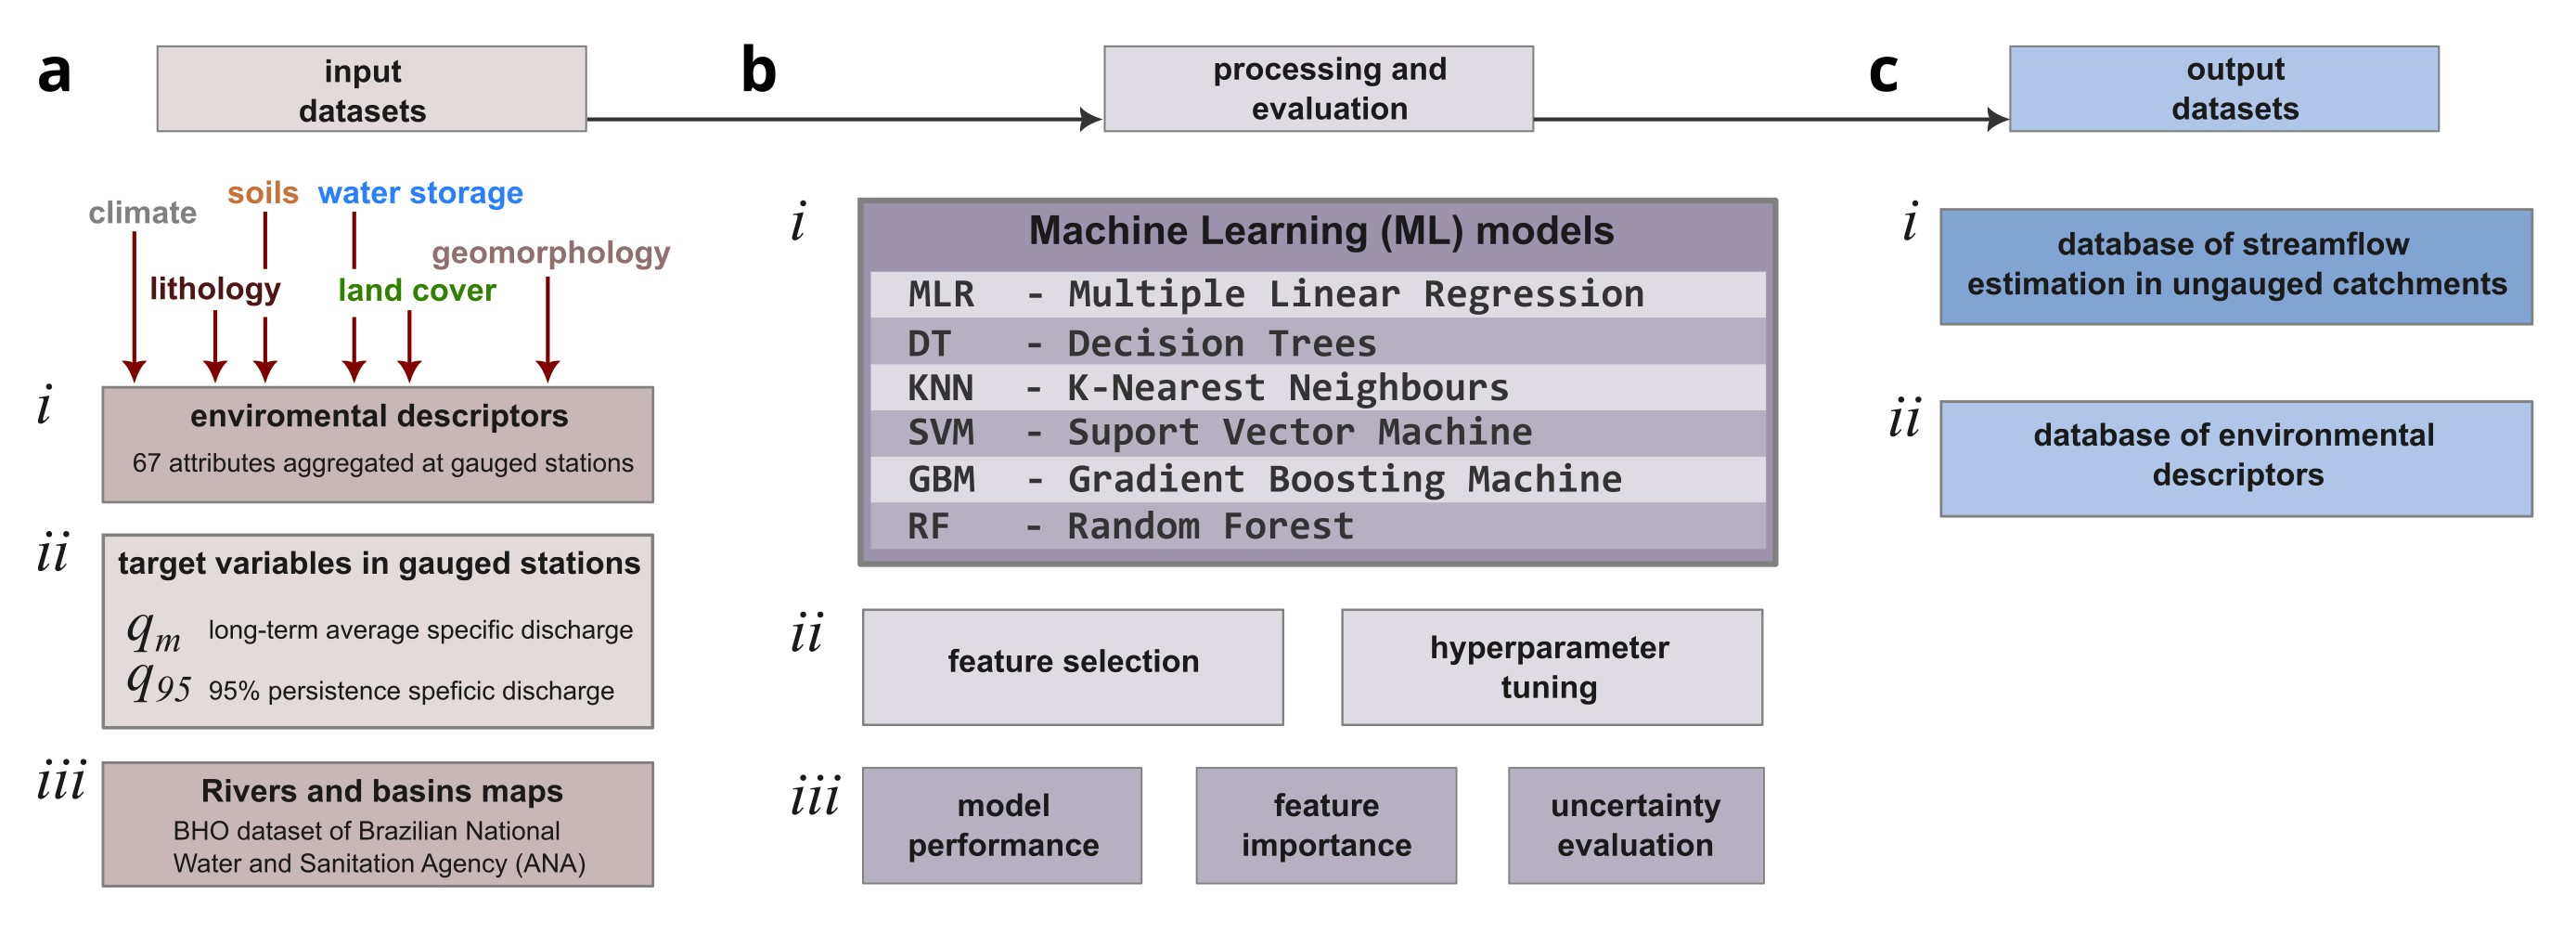
\includegraphics[width=0.98\linewidth]{figs/methods.jpg}    
	\caption[General methodology framework]
	{\textbf{---\;General Workflow for the Proposed Approach}. 
		\textbf{a}\,--\,The workflow began by establishing input datasets. These included environmental descriptors (detail \textrm{\textit{i}}, encompassing data related to climate, soils, lithology, water storage, land cover, and geomorphology), the target variables at gauged stations (detail \textrm{\textit{ii}}, covering long-term average specific discharge $q_m$ and 95\% persistence specific discharge $q_{95}$), and river and basin maps for regionalization (detail \textrm{\textit{iii}}, with data sourced from the BHO dataset \cite{ana2017}).
		\textbf{b}\,--\,The second stage entailed processing and evaluating results. Six Machine Learning models (detail \textrm{\textit{i}}) were fitted following feature selection and hyperparameter tuning (detail \textrm{\textit{ii}}). The evaluation (detail \textrm{\textit{iii}}) focused on model performance metrics, feature importance, and uncertainty assessment.	
        \textbf{c}\,--\,Finally, the output dataset comprised the database of streamflow estimates in ungauged catchments across the entire Brazilian territory (detail \textrm{\textit{i}}) and a consolidated database for the environmental descriptors (detail \textrm{\textit{ii}}).	
	}
	\label{fig:methods}  % use qualitative label                      
\end{figure}

\par In our study, we structured our workflow to encompass a comprehensive approach to data collection, preparation, processing, modeling, and evaluation. This section and Figure \ref{fig:methods} aims to provide an overview of our workflow, uncovering each step and the methodologies employed. In the following sections, we will delve deeper into each of these steps, offering detailed insights into our methodologies and the rationale behind our choices.

\par We initiated our process with data collection and preparation, focusing on gathering a wide range of environmental descriptors that could influence hydrological responses. These descriptors, including climate, water storage, landscape composition, and topography, were meticulously selected and normalized for consistency across different river basins. For data processing and modeling, we utilized the scikit-learn library in Python. An essential part of our methodology was feature selection, aiming to remove multicollinearity and enhance model performance. We adopted hierarchical clustering to identify and group similar features. This step was crucial for ensuring model efficiency and accuracy.

\par We then applied a K-Fold cross-validation approach for training and validating our machine learning models, which included Multiple Linear Regression (MLR), Decision Trees (DT), K-Nearest Neighbors (KNN), Support Vector Machines (SVM), Gradient Boosting Machines (GBM), and Random Forest (RF). Each model underwent hyperparameter tuning, followed by evaluation using metrics such as BIAS, RMSE, and \( R^2 \). The hyperparameter tuning was executed using a randomized search grid cross-validation method, ensuring we found the most effective model parameters. An integral part of our workflow was the uncertainty analysis, conducted using the \texttt{CV+} method from the Mapie Python library, which estimates prediction intervals around test data predictions. This robust approach was critical for ensuring the reliability of our models. Furthermore, we assessed the importance of each predictor using permutation feature importance. This method helped us understand the impact of each variable on our models' predictions, enhancing our interpretation and understanding of the models. Finally, the model evaluation phase involved analyzing the outcomes of each fold in the 10-fold cross-validation process. We used statistical measures to evaluate the performance of our models, providing a comprehensive understanding of their effectiveness and reliability. 

% Target variables and delimitation of river basins
\subsection{Target variables and river basins} \label{sec:methods:target}

\par Two target variables were analyzed in this study that reflect the long-term behaviour of a catchment within the ambit of water resource management. These variables are the long-term average discharge ($Q_{m}$) and the discharge with a 95\% persistence rate ($Q_{95}$), calculated from daily series of river gauge stations obtained from the Hidroweb database of ANA. Only stations with data series spanning from Jan/1980 to Dec/2014 and containing at least 20 years of data were considered. Furthermore, only stations without significant effects of artificial regulation and/or gross errors in the data series, or of special interest to ANA, were considered. An analysis of estimation errors in long-term discharge associated with sample variability  has demonstrated that estimates based on 20 years of data exhibit errors lower than 5\% in $Q_{m}$ and lower than 15\% in $Q_{95}$ when compared to series of 30 to 35 years in most evaluated cases (\cite{collischonn2021}). Considering these criteria, 1069 stream gauge stations were identified, presented in Figure \ref{fig:rivers}a. For the training and evaluation of the models, the variables used were expressed in specific units ($q_{m}$ and $q_{95}$), dividing the values of $Q_{m}$ and $Q_{95}$ by the area of the upstream basin of each station. Figure \ref{fig:rivers}b illustrate the role of the target variables $q_{m}$ and $q_{95}$ to understand the structure and diversity of  catchment long term behaviour from the inspection of flow duration curves across the Brazilian territory. 

\par Drainage basins were delimited using the Ottocodified hydrological database (\texttt{BHO}) version 5k (\cite{ana2017}), which was produced by the digitalization of cartographic hydrology data from field surveys produced through decades of development efforts by the Brazilian National Water and Sanitation Agency (ANA) and the Brazilian Institute of Geography and Statistics (IBGE), containing valuable information on Brazilian rivers . It consists of unit catchments, in terms of polygons and river lines, with several topological information, making it easy to delimit drainage areas based on the Pfafstetter coding system (\cite{teixeira2022}). For each stream gauge it was defined which unit catchment comprised it (outlet), and them identified all of its upstream unit catchments following the Pfafstetter system. Then, a union operation was performed in all of the polygons, forming the river basin of that station, which was used to collect all data from environmental descriptors. From the \texttt{BHO} dataset, it was also taken drainage area information to be used as a potential predictor.

\begin{figure}[t!] % place figure in the page
	\centering                                       
	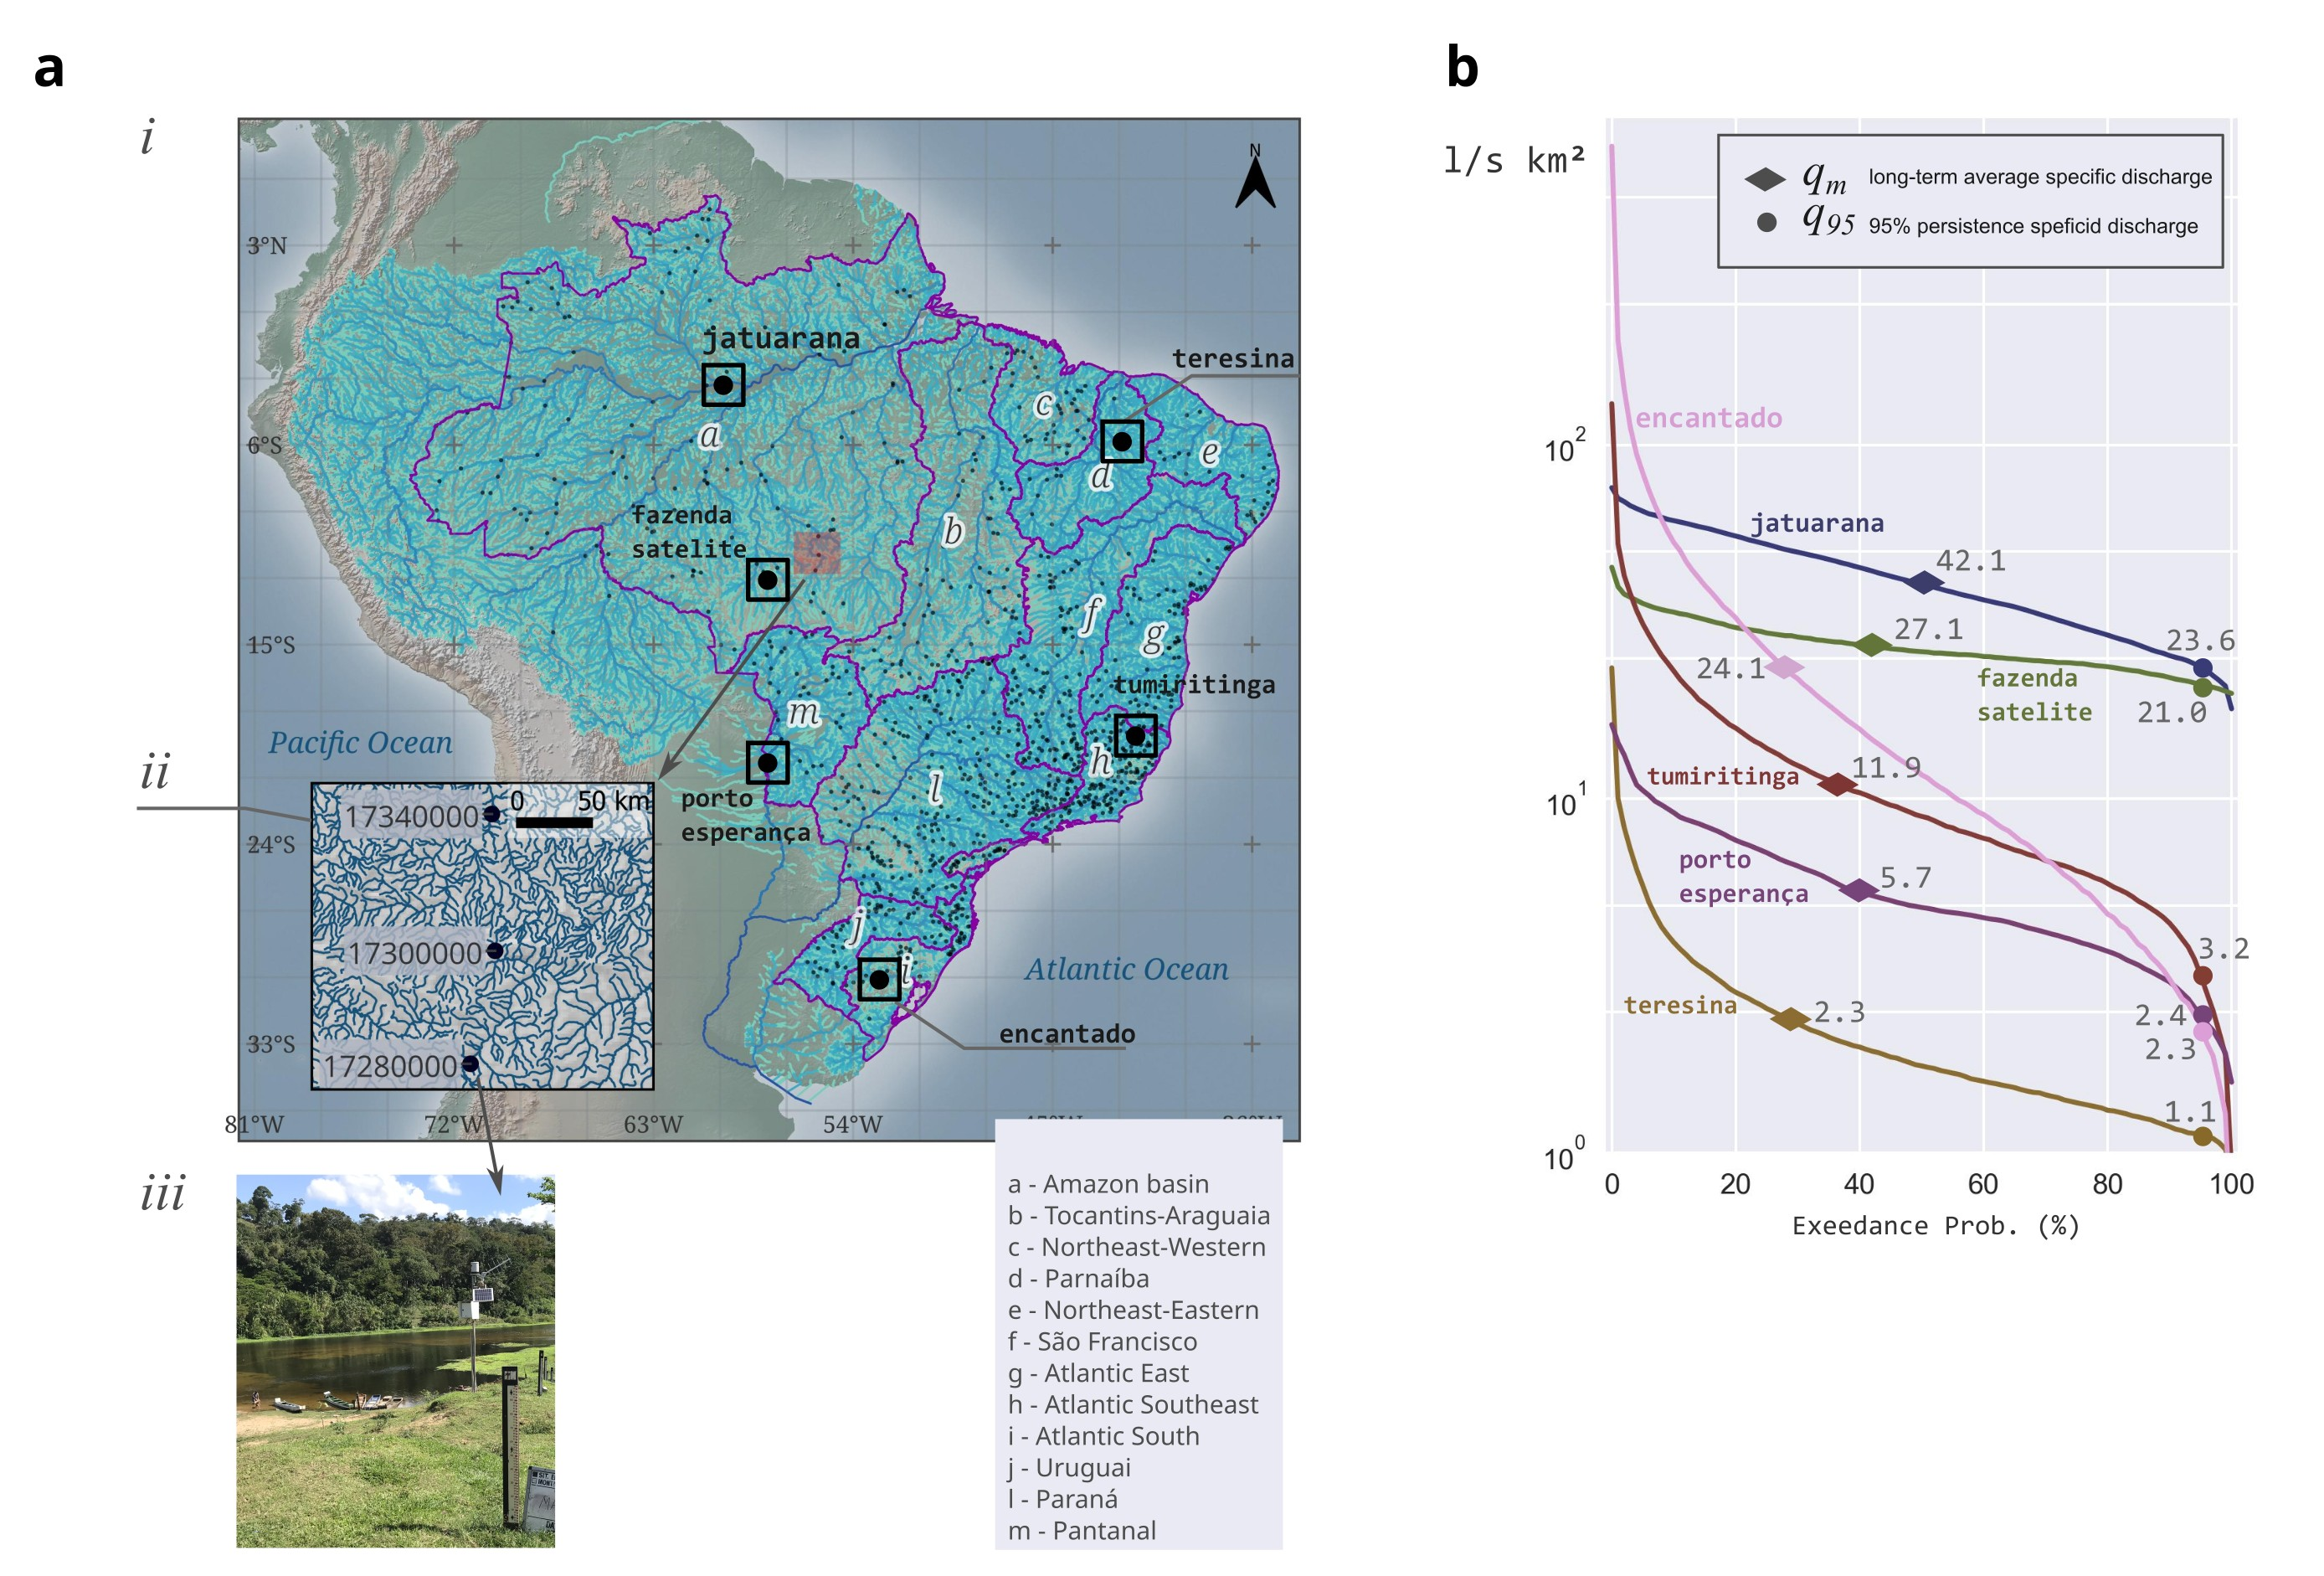
\includegraphics[width=0.98\linewidth]{figs/target.jpg}    
	\caption[Target variables]
	{\textbf{---\;Target variables and locations of the stream gauges used to evaluate the \texttt{ML} models}.
	\textbf{a}\,--\,Map in detail \textrm{\textit{i}} displays the full extent of the Ottocodified hydrological database (\texttt{BHO}) version 5k (\cite{ana2017}), across all Brazilian basins (including contributing areas from neighbouring countries in South America). Detail \textrm{\textit{ii}} uncovers the mapped drainged network and gauged stations. Detail \textrm{\textit{iii}} illustrate the gauged stations operated by Brazilian Geological Survey.
	\textbf{b}\,--\,Illustration of the target variables $q_{m}$ and $q_{95}$ (specific discharge) in flow duration curves in selected stations across the Brazilian territory. The selected stations are also highlighted in \textbf{a}.
	}
    \label{fig:rivers}            
\end{figure}

% Environmental descriptors
\subsection{Environmental descriptors datasets} \label{sec:methods:data}

\par We evaluated 67 variables of environmental descriptors with potential to influence the hydrological response of a river basin. These variables were selected based on environmental characteristics with potential to describe catchment behaviour and, therefore, streamflow response. Here, they were grouped in domains of climate, water storage, landscape composition, and topography. A summary of all variables is presented in Table \ref{tab:predictors}. Next, a brief description of the variables and datasets used is given.

% Insert Table 1
\begin{table}[t]
\centering
\tiny
\rowcolors{2}{white}{rowgray}
\begin{tabular}{p{0.5cm}p{1cm}p{2cm}p{3.5cm}p{5cm}}
\toprule
\textbf{Code} & \textbf{Notation} & \textbf{Domain} & \textbf{Description} & \textbf{Source} \\
\midrule
V1 & $P_{avg}$ & Climate & Precipitation average & Remote Sensing -- \texttt{IMERG}\\
V2 & $P_{min}$ & Climate & Precipitation minimum & Remote Sensing -- \texttt{IMERG}\\
V3 & $P_{max}$ & Climate & Precipitation maximum & Remote Sensing -- \texttt{IMERG}\\
V4 & $T_{avg}$ & Climate & Temperature average & Remote Sensing -- \texttt{MODIS}\\
V5 & $T_{min}$ & Climate & Temperature minimum & Remote Sensing -- \texttt{MODIS}\\
V6 & $T_{max}$ & Climate & Temperature maximum & Remote Sensing -- \texttt{MODIS}\\
V7 & $ET_{avg}$ & Climate & Evapotranspiration average & Remote Sensing -- \texttt{MODIS}\\
V8 & $ET_{min}$ & Climate & Evapotranspiration minimum & Remote Sensing -- \texttt{MODIS}\\
V9 & $ET_{max}$ & Climate & Evapotranspiration maximum & Remote Sensing -- \texttt{MODIS}\\
V10 & $PET_{avg}$ & Climate & Potential Evapot. average & Remote Sensing -- \texttt{MODIS}\\
V11 & $PET_{min}$ & Climate & Potential Evapot. minimum & Remote Sensing -- \texttt{MODIS}\\
V12 & $PET_{max}$ & Climate & Potential Evapot. maximum & Remote Sensing -- \texttt{MODIS}\\
V13 & $RS$ & Water Storage & Reservoir storage & \texttt{SIN}  -- \cite{ana2021}\\
V14 & $GW$ & Water Storage & Groundwater storage & \texttt{MGB-SA} -- \cite{siqueira2018}\\
V15 & $SW$ & Water Storage & Surface water & \texttt{MGB-SA} -- \cite{siqueira2018}\\
V16 & $SM$ & Water Storage & Soil Moisture & \texttt{GLDAS} -- \cite{rodell2004}\\
V17 & $TWS$ & Water Storage & Total water storage & Remote Sensing -- \texttt{GRACE} and \texttt{GRACE-FO}\\
V18 & $LT_{Ev}$ & Lithology & Evaporites & \texttt{GLiM}  -- \cite{hartmann2012}\\
V19 & $LT_{Ig}$ & Lithology & Ice and Glaciers & \texttt{GLiM}  -- \cite{hartmann2012}\\
V20 & $LT_{Mt}$ & Lithology & Metamorphics & \texttt{GLiM}  -- \cite{hartmann2012}\\
V21 & $LT_{Nd}$ & Lithology & No Data & \texttt{GLiM}  -- \cite{hartmann2012}\\
V22 & $LT_{Pa}$ & Lithology & Acid plutonic rocks & \texttt{GLiM}  -- \cite{hartmann2012}\\
V23 & $LT_{Pb}$ & Lithology & Basic plutonic rocks & \texttt{GLiM}  -- \cite{hartmann2012}\\
V24 & $LT_{Pi}$ & Lithology & Intermediate plutonic rocks & \texttt{GLiM}  -- \cite{hartmann2012}\\
V25 & $LT_{Py}$ & Lithology & Pyroclastics & \texttt{GLiM}  -- \cite{hartmann2012}\\
V26 & $LT_{Sc}$ & Lithology & Carbonate sed. rocks & \texttt{GLiM}  -- \cite{hartmann2012}\\
V27 & $LT_{Sm}$ & Lithology & Mixed sedimentary rocks & \texttt{GLiM}  -- \cite{hartmann2012}\\
V28 & $LT_{Ss}$ & Lithology & Siliciclastic sed. rocks & \texttt{GLiM}  -- \cite{hartmann2012}\\
V29 & $LT_{Su}$ & Lithology & Unconsolidated sediments & \texttt{GLiM}  -- \cite{hartmann2012}\\
V30 & $LT_{Va}$ & Lithology & Acid volcanic rocks & \texttt{GLiM}  -- \cite{hartmann2012}\\
V31 & $LT_{Vb}$ & Lithology & Basic volcanic rocks & \texttt{GLiM}  -- \cite{hartmann2012}\\
V32 & $LT_{Vi}$ & Lithology & Intermediate volcanic rocks & \texttt{GLiM}  -- \cite{hartmann2012}\\
V33 & $LT_{Wb}$ & Lithology & Water Bodies & \texttt{GLiM}  -- \cite{hartmann2012}\\
V34 & $LT_{Pr}$ & Lithology & Precambrian rocks & \texttt{GLiM}  -- \cite{hartmann2012}\\
V35 & $LT_{Ev}$ & Lithology & Evaporites & \texttt{GLiM}  -- \cite{hartmann2012}\\
\bottomrule
\end{tabular}
\caption{\textbf{(first part)} Environmental predictors used as input for the \texttt{ML} models.}
\label{tab:predictors}
\end{table}

\begin{table}[t]
\centering
\tiny
\rowcolors{2}{white}{rowgray}
\begin{tabular}{p{0.5cm}p{1cm}p{2cm}p{3.5cm}p{5cm}}
\toprule
\textbf{Code} & \textbf{Notation} & \textbf{Domain} & \textbf{Description} & \textbf{Source} \\
\midrule
V36 & $S_{d}$ & Soil & Soil density (g/kg) & \texttt{OpenLandMap} -- \cite{hengl2017}\\
V37 & $S_{cly}$ & Soil & Soil organic content (g/g) & \texttt{OpenLandMap} -- \cite{hengl2017}\\
V38 & $S_{org}$ & Soil & Soil sand content (g/g) & \texttt{OpenLandMap} -- \cite{hengl2017}\\
V39 & $S_{snd}$ & Soil & Soil clay content (g/g) & \texttt{OpenLandMap} -- \cite{hengl2017}\\
V40 & $S_{Cl}$ & Soil & Clay & \texttt{OpenLandMap}  -- \cite{hengl2017}\\
V41 & $S_{SiCl}$ & Soil & Silty clay & \texttt{OpenLandMap}  -- \cite{hengl2017}\\
V42 & $S_{SaCl}$ & Soil & Sandy clay & \texttt{OpenLandMap}  -- \cite{hengl2017}\\
V43 & $S_{ClLo}$ & Soil & Clay loam & \texttt{OpenLandMap}  -- \cite{hengl2017}\\
V44 & $S_{SiClLo}$ & Soil & Silty clay loam & \texttt{OpenLandMap}  -- \cite{hengl2017}\\
V45 & $S_{SaClLo}$ & Soil & Sandy clay loam & \texttt{OpenLandMap}  -- \cite{hengl2017}\\
V46 & $S_{Lo}$ & Soil & Loam & \texttt{OpenLandMap}  -- \cite{hengl2017}\\
V47 & $S_{SiLo}$ & Soil & Silty loam & \texttt{OpenLandMap}  -- \cite{hengl2017}\\
V48 & $S_{SaLo}$ & Soil & Sandy loam & \texttt{OpenLandMap}  -- \cite{hengl2017}\\
V49 & $S_{Si}$ & Soil & Silt & \texttt{OpenLandMap}  -- \cite{hengl2017}\\
V50 & $S_{LoSa}$ & Soil & Loamy sand & \texttt{OpenLandMap}  -- \cite{hengl2017}\\
V51 & $S_{Sa}$ & Soil & Sand & \texttt{OpenLandMap}  -- \cite{hengl2017}\\
V52 & $LC_{f}$ & Land Cover & Forest & \texttt{Mapbiomas} -- \cite{souza2020} and \texttt{MODIS}\\
V53 & $LC_{g}$ & Land Cover & Grassland & \texttt{Mapbiomas} -- \cite{souza2020} and \texttt{MODIS}\\
V54 & $LC_{c}$ & Land Cover & Agriculture & \texttt{Mapbiomas} -- \cite{souza2020} and \texttt{MODIS}\\
V55 & $LC_{p}$ & Land Cover & Semi-permeable & \texttt{Mapbiomas} -- \cite{souza2020} and \texttt{MODIS}\\
V56 & $LC_{w}$ & Land Cover & Water & \texttt{Mapbiomas} -- \cite{souza2020} and \texttt{MODIS}\\
V57 & $ELV_{avg}$ & Geomorphology & Elevation average & \texttt{MERIT} -- \cite{yamazaki2017}\\
V58 & $ELV_{std}$ & Geomorphology & Elevation SD & \texttt{MERIT} -- \cite{yamazaki2017}\\
V59 & $SLP_{avg}$ & Geomorphology & Slope average & \texttt{MERIT} -- \cite{yamazaki2017}\\
V60 & $SLP_{std}$ & Geomorphology & Slope SD & \texttt{MERIT} -- \cite{yamazaki2017}\\
V61 & $HND_{avg}$ & Geomorphology & HAND average & \texttt{MERIT-Hydro} -- \cite{yamazaki2019}\\
V62 & $HND_{std}$ & Geomorphology & HAND SD & \texttt{MERIT-Hydro} -- \cite{yamazaki2019}\\
V63 & $DD$ & Geomorphology & Drainage density & \texttt{MERIT-Hydro} -- \cite{yamazaki2019}\\
V64 & $A$ & Geomorphology & Upstream area & \texttt{MERIT-Hydro} -- \cite{yamazaki2019}\\
V65 & $TC_{wet}$ & Geomorphology & Wetland & derived from \texttt{MERIT-Hydro}\\
V66 & $TC_{hsp}$ & Geomorphology & Hillslope & derived from \texttt{MERIT-Hydro}\\
V67 & $TC_{plt}$ & Geomorphology & Plateau & derived from \texttt{MERIT-Hydro}\\
\bottomrule
\end{tabular}
\caption*{\textbf{Table \ref{tab:predictors} (continued)} Environmental predictors used as input for the \texttt{ML} models.}
\end{table}

\par Climate-related variables such as precipitation, temperature, evapotranspiration, and potential evapotranspiration, were normalized to monthly averages from 2001 to 2020 for each river basin, using minimum, maximum, and average values. Precipitation, crucial for streamflow in hydrological basins, was sourced from the Integrated Multi-Satellite Retrievals for \texttt{GPM} (\texttt{IMERG}), a product of \texttt{NASA} and \texttt{JAXA} (\cite{huffman2020}). \texttt{IMERG} provides high-resolution global precipitation estimates, combining data from satellites like \texttt{TRMM} (\cite{huffman2007}) and the \texttt{GPM} mission (\cite{skofronick2017}). Other essential variables, such as land surface temperature (\textit{T}), evapotranspiration (\textit{ET}), and potential evapotranspiration (\textit{PET}), were collected from the Moderate Resolution Imaging Spectroradiometer (\texttt{MODIS}) products (\cite{mu2007, mu2011i}), derived from the Terra and Aqua satellites. These variables play a significant role in the water loss processes and are key to understanding streamflow responses in basins.

\par Different components of water storage such as groundwater, soil moisture, surface water, and reservoir water were also included in the list of enviromental descriptors. These variables substantially impact streamflow response in Brazilian catchments (\cite{barbedo2022b}). These components were considered as potential predictors for \( Q_{m} \) and \( Q_{95} \), with data collection methods detailed in \cite{barbedo2022a}. Total water storage data was derived from the Gravity Recovery and Climate Experiment (\texttt{GRACE}) and its follow-up mission \texttt{GRACE-FO}, which measure changes in Earth's gravity field due to water mass distribution shifts (\cite{landerer2020, tapley2004}). Reservoir storage information came from the Brazilian National Interconnected System (SIN), providing insights into reservoir capacities and water levels (\cite{ana2021}). Surface water storage data was acquired from the \texttt{MGB-SA} hydrological model, a physically-based framework that simulates the hydrological cycle of Brazilian river basins and includes rivers, lakes, and wetlands (\cite{siqueira2018}). Soil moisture data, crucial for understanding plant water uptake, was sourced from the Global Land Data Assimilation System (\texttt{GLDAS}), which assimilates various data to estimate soil moisture globally, particularly in the root zone (\cite{rodell2004}).

\par Lithology, Soil, and Land Cover were taken as key landscape composition variables. These variables, often classified into distinct types, were analyzed based on their percentage occupancy within basin boundaries, with numerical soil variables averaged over basin areas. Lithology, influencing water movement through varying capacities, permeability, and porosity, was derived from the Global Lithological Map (\texttt{GLiM}) database (\cite{hartmann2012}). This database, at a 50km resolution, amalgamates geological information from various sources to categorize the Earth's surface into ten lithological classes, including sedimentary, volcanic, plutonic, metamorphic rocks, and unconsolidated deposits. Soil properties, essential in dictating streamflow responses, were sourced from the \texttt{OpenLandMap} database (\cite{hengl2017}). This comprehensive database offers detailed global soil information at 250m resolution, including texture, organic matter content, and pH, utilizing a blend of soil maps and advanced modelling. Land cover, a crucial factor in the hydrological cycle, was analyzed based on its influence on processes like interception, infiltration, and runoff. We used data from the \texttt{Mapbiomas} database (\cite{souza2020}) for Brazilian territory and the \texttt{MODIS} dataset (\cite{friedl201}) for other areas. Both databases' original land cover classes were simplified into five categories: forests, grasslands, agriculture, semi-permeable regions, and water bodies, facilitating cross-regional analysis and comparison. \texttt{Mapbiomas} offers high-resolution land use and cover change data for Brazil, while \texttt{MODIS} provides global land cover information, making them invaluable for understanding landscape changes and their impact on streamflow.

\par Geomorphological variables were recognized as pivotal in understanding the distribution of hydrological conditions, since they dictate water and energy movement across the landscape. Hence, variables derived from a digital elevation model (\texttt{DEM}) were used, with some requiring minimal processing, like elevation and slope, and others needing more complex procedures, such as drainage networks and terrain classes. Elevation and slope data for each river basin, including averages and standard deviations, were obtained from the \texttt{MERIT-DEM} product (\cite{yamazaki2017}). This global digital elevation model, with a resolution of approximately 90 meters at the equator, corrects major errors from existing \texttt{DEM} datasets. For drainage information, crucial in predicting streamflow, we used the Topographic Position based Stream definition (\texttt{TPS}) (\cite{barbedo2022b}) to generate a stream mask using \texttt{MERIT-DEM} and \texttt{MERIT-Hydro} (\cite{yamazaki2019}). This facilitated the creation of a Height Above Nearest Drainage (\texttt{HAND}) map (\cite{nobre2011, renno2008}), providing insights into drainage density and water table depth across river basins in the \texttt{BHO} dataset. We also classified the landscape into three hydrological terrain classes: wetlands, hillslopes, and plateaus, based on drainage locations and \texttt{DEM} data (\cite{gao2014, gharari2011, savenije2010}). Wetlands, typically saturated areas, were identified using a \texttt{HAND} threshold, hillslopes by slope thresholds indicating faster water movement and erosion, and plateaus as areas generally higher and flatter, crucial for groundwater recharge. This classification provided valuable information for various hydrological applications.

% Machine Learning algorithms
\subsection{Machine Learning models} \label{sec:methods:ml}

\par As outlined in Table \ref{tab:algorithms}, six machine learning (\texttt{ML}) models for regression were tested in this study. They are presented in this section aggregated in ascending order of complexity and computational demand, with the simpler models (first two) used as benchmarks for the more complex ones. Multiple Linear Regression (\texttt{MLR}) and Decision Trees (\texttt{DT}) were the first two models tested, followed by K-Nearest Neighbors (\texttt{KNN}), Support Vector Machines (\texttt{SVM}), Gradient Boosting Machine (\texttt{GBM}), and Random Forest (\texttt{RF}). For a comprehensive understanding of the models, including their mathematical foundations, see \cite{kuhn2013} and \cite{shalev2014}. 

% Insert Table 1
\begin{table}[h]
    \centering
    \tiny
    \rowcolors{2}{white}{rowgray}
\begin{tabular}{p{4cm}p{1.5cm}p{1.5cm}p{2cm}p{1cm}p{1cm}}
\toprule
\textbf{Model}& \textbf{Complexity} & \textbf{Linear} & \textbf{Parametric} & \textbf{Missing Data} & \textbf{Intensive} \\
\midrule
Multiple Linear Regression (\texttt{MLR}) & Low & Linear & Parametric & \texttimes & \texttimes \\
Decision Trees (\texttt{DT}) & Low& Non-linear & Non-parametric & $\checkmark$ & \texttimes \\
K-Nearest Neighbours (\texttt{KNN}) & Medium & Non-linear & Non-parametric & \texttimes & $\checkmark$ \\
Support Vector Machines (\texttt{SVM}) & Medium& Non-linear & Parametric & \texttimes & $\checkmark$ \\
Gradient Boosting Machine (\texttt{GBM}) & High & Non-linear & Parametric & \texttimes & $\checkmark$ \\
Random Forest (\texttt{RF}) & High & Non-linear & Non-parametric & $\checkmark$ & $\checkmark$ \\
\bottomrule
\end{tabular}
\caption{Summary of Machine Learning models applied in the study.}
\label{tab:algorithms}
\end{table}

\par As mentioned above, we used Multiple Linear Regression (MLR) and Decision Trees (DT) as benchmark models. MLR is a straightforward machine learning model that presumes a proportional relationship between a dependent variable and all independent variables. Its objective is to identify a best-fit line for accurate prediction of the dependent variable, utilizing the Ordinary Least Squares method to minimize prediction errors. On the other hand, DT is a non-parametric model predicting the target variable's value through a tree-like structure. It segments data based on feature values until a specific criterion is reached, with predictions derived from the data characteristics of the leaf nodes. While DTs are interpretable and adept at handling complex feature interactions and missing data, they are susceptible to overfitting and can generate overly complex trees. In practice, this is often mitigated by using ensemble models like Random Forest and Gradient Boosting Machines.

\par In the intermediate complexity stage of our study, we employed K-Nearest Neighbours (\texttt{KNN}) and Support Vector Machines (\texttt{SVM}). \texttt{KNN} is a non-parametric model that bases its predictions on the $K$ nearest data points in the training set, without making assumptions about data distribution. It's applicable for both regression and classification, with predictions relying on the majority class among the $K$ neighbors. While \texttt{KNN} is straightforward to implement and adept at capturing complex feature relationships, it is computationally intensive and sensitive to hyperparameters like the value of $K$ and the chosen distance metric. \texttt{SVM}, on the other hand, is a linear model designed to find the optimal hyperplane that distinctively classifies data into different groups. It focuses on maximizing the margin between this hyperplane and the nearest data points from each class. Capable of managing non-linear relationships through kernel functions, which project data into higher dimensions, \texttt{SVM} is essential in fields like image and text classification, and bioinformatics. Nonetheless, its effectiveness hinges on the correct choice of hyperparameters like the kernel function and regularization parameter, and it requires significant computational resources for large datasets.

\par Finally we utilized the more complex Gradient Boosting Machines (\texttt{GBM}) and Random Forest (\texttt{RF}). \texttt{GBM} is an ensemble approach that amalgamates several weak models to form a potent predictive model. It progressively refines weak models based on the residual errors from preceding iterations, culminating in a prediction that combines all these models' outputs. \texttt{GBM} efficiently manages intricate feature interactions and generally exhibits greater resistance to overfitting compared to other tree-based models. However, it requires careful hyperparameter tuning, particularly in learning rate and tree count, and can be computationally demanding for extensive datasets. \texttt{RF}, another ensemble model, integrates multiple decision trees to forge a precise and robust prediction tool. It selects random feature and data point subsets for each tree, enhancing feature interaction capture and reducing overfitting risks. Predictions result from an aggregate of all trees' outputs, enhancing both accuracy and generalizability. While \texttt{RF} adeptly handles missing values and outliers, making it a popular choice in various applications, it also demands significant computational resources and offers less interpretability than individual decision trees.

% Feature selection
\subsection{Feature selection} \label{sec:methods:selection}

\par Hierarchical clustering was employed for feature selection, as described by \cite{johnson1967}. This technique involves grouping similar data points into clusters, visualized through a dendrogram, a tree-like structure. In feature selection, hierarchical clustering aids in identifying groups of similar features for potential combination or removal. The process began with the creation of a correlation matrix, using the Spearman correlation coefficient to capture non-linear relationships among variables. This matrix displayed pairwise correlations between all features. Following this, features were clustered based on their pairwise correlation distance. The dendrogram helped in deciding the level at which to cut and form the final feature clusters. The number of clusters chosen depended on the chosen dendrogram cut-off distance.

\par Feature selection within each cluster was then carried out. The representative feature was determined as the one with the highest correlation to the target variable. This approach varied for each target variable (\( q_{m} \) and \( q_{95} \)), ensuring the selection of the most relevant features. The process of selecting the cutting threshold for the dendrogram was iterative, focusing on model performance and ensuring the remaining features were representative of the dataset. The criterion set was to maintain features with pairwise Spearman absolute correlation below 0.7. This method ensured the inclusion of the most representative variables while avoiding multi-collinearity, balancing representativeness and analytic integrity.

\subsection{Hyperparameter tuning} \label{sec:methods:tuning}

\par The process of hyperparameter tuning was performed using a randomized search grid cross validation approach (\cite{bergstra2012} ). The approach consists of randomly  sampling hyperparameters from the \texttt{ML} model using a specified distribution and evaluating the performance of the model for each set of hyperparameters using cross-validation (here, another 5 folds were used on the training set for each outer iteration). The best set of hyperparameters is then selected based on the model's performance, here chosen to be evaluated using $R^2$ (explained in next section). The randomized search grid approach has several advantages over a traditional grid search approach (\cite{bergstra2012}), which involves evaluating every possible combination of hyperparameters. First, it is computationally efficient because it only evaluates a subset of the possible hyperparameter combinations, reducing the time required to find the best set of hyperparameters. Additionally, it can often find better hyperparameter settings than grid search because it is not constrained to a predefined grid of values and can search a broader range of hyperparameter values. The set of distributions for each hyperparameter of each \texttt{ML} model is presented in Table 8. It is important to note that, in order to reduce complexity, only the most sensible hyperparameters of the \texttt{ML} models were tested, the others remaining in default mode from the scikit-learn Python library. After the hyperparameters of the model were defined, the selected optimal model was fitted to the training data, and used to predict the results on the test data.

% Insert Table
\begin{table}[t]
\centering
\tiny
\rowcolors{2}{white}{rowgray}
\begin{tabular}{p{3cm}p{3cm}p{3cm}}
\toprule
\textbf{Model} & \textbf{Parameter} & \textbf{Range$^*$}\\
\midrule
\texttt{MLR} & -- & --\\
\texttt{DT} & \texttt{max depth} & int(2, 20)\\
\texttt{DT} & \texttt{min samples leaf} & int(5, 100) \\
\texttt{KNN} & \texttt{leaf size} & int(1, 50) \\
\texttt{KNN} & \texttt{n neighbors} & int(1, 30) \\
\texttt{KNN} & \texttt{p} & int(1,5) \\
\texttt{SVM} & \texttt{gamma} & dbl(0.0001, 1)\\
\texttt{SVM} & \texttt{C} & dbl(1, 100)\\
\texttt{GBM} & \texttt{n estimators} & int(1, 500)\\
\texttt{GBM} & \texttt{max leaf nodes} & int(2, 100)\\
\texttt{GBM} & \texttt{learning rate} & dbl(0.01, 1)\\
\texttt{RF} & \texttt{n estimators} & int(1, 500)\\
\texttt{RF} & \texttt{max leaf nodes} & int(2, 100)\\
\bottomrule
\end{tabular}
\smallskip
    \parbox[t]{10cm}{\footnotesize
      \textit{$^*$ Legend: \\
      int: integer precision. \\ 
      dbl: double precision.}
    }
\caption{Ranges of hyperparameter values for tuning each \texttt{ML} model.}
\label{tab:parameters}
\end{table}

\subsection{Uncertainty evaluation} \label{sec:methods:uncert}

\par The uncertainty assessment of machine learning models was conducted to gain insights into the distribution of residuals from the obtained fits. The residuals were calculated using a linear model with additive error ($\epsilon$), where the predicted values $M$ are precisely the observed values $O$, that is, $M = O + \epsilon$. A qualitative visual analysis was then performed for each fit, aided by various plots: residual plot, residual histogram, Quantile-Quantile plot, and cumulative variance plot. Both the residual plot and histogram aided in evaluating hypotheses about the error structure of the fitted models. The Quantile-Quantile plot, in addition to aiding in structural interpretation, helped qualitatively assess deviations from normality (the straighter the distribution of plotted quantiles, the smaller the deviation from normality). The cumulative variance plot contributed to assessing the stability of the error, a fundamental component in hypothesizing about the error structure.

\par Once a qualitative analysis of the uncertainty was established, three hypotheses about the residual structure (for each fitted model and target variable) were evaluated using the Kolmogorov-Smirnov test (\cite{massey1951}). The first hypothesis considered was simply that the error of the fits follows a normal distribution. Given the unlikelihood of this hypothesis from the outset, two more variable transformations were considered. The second hypothesis posited the normality of the error following a logarithmic transformation of the observed and predicted variables. Finally, the third hypothesis considered was the normality of the error following a square root transformation of the observed and predicted variables. In addition to the Kolmogorov-Smirnov test, these hypotheses were also visually evaluated, with particular attention given to those not refuted.

\par >>todo: evaluate presenting old methods

\par \textcolor{red}{We conducted an uncertainty analysis using the \texttt{CV+} method from the Mapie Python library (https://mapie.readthedocs.io/en/latest/index.ht\texttt{ML}). This method, analogous to the Jackknife+ method as described by \cite{barber2021}, differs primarily in its use of K-Fold Cross Validation instead of Leave-One-Out Cross Validation (LOOCV). The \texttt{CV+} method is designed to estimate prediction intervals centered around the test data predictions using a robust approach. The process begins by splitting the training data into \( K \) equal-sized subsets. For each subset, a regression function is fitted on the training set, excluding the corresponding \( k^{th} \) fold. Then, a conformity score, which is the absolute residual between the observation and the prediction from the \( k^{th} \) model, is computed for each point in the \( k^{th} \) fold. Lastly, these regression functions are employed to estimate the prediction intervals on the test data. This approach guarantees a coverage level higher than \( 1- 2\alpha \) for a targeted coverage of \( 1- \alpha \), operating without any a priori assumptions on the distribution of the data. For our specific analysis, we set \( K \) to 5 and \( \alpha \) to 0.05, following these parameters to ensure a robust estimation of uncertainty.}  

\subsection{Feature importance} \label{sec:methods:importance}

\par The importance of each predictor in the Machine Learning Model (\texttt{MLM}) was evaluated using permutation feature importance, a method outlined by \cite{altmann2010}. This approach involves assessing the model's performance when a single feature is randomly shuffled, with the importance measured by the loss in an accuracy metric, such as \( R^2 \). By shuffling a variable to random values, the resultant decrease in performance metric value indicates the importance of that variable. Permutation feature importance is particularly useful in analyzing black-box models, where it's challenging to discern how specific variables impact results. It offers a consistent standard for evaluating different models and accounts for all interactions between features, though it doesn't elucidate the nature of the relationship with the target variable.

\par The process starts by selecting a performance metric for the model, in our case \( R^2 \). The model's performance is then assessed on the test set to establish a baseline. Following this, the values of a single feature are permuted in the validation set, and the model's performance is re-evaluated. This process involves random shuffling of one feature while keeping other features and the target variable unchanged. The importance of a feature is determined by the difference in model performance with original and permuted feature values. This procedure is repeated for all features in the dataset, multiple times for each feature (we used n=10), to ensure that the model's performance isn't influenced by random data. The feature's importance score is then derived from the average performance decrease across these iterations. This method is critical, especially in cases where correlated features are present, underscoring the need to address multicollinearity before the processing phase.

\subsection{Model evaluation} \label{sec:methods:eval}

\par After the processes covered in the previous section were performed in each one of the 10-fold combinations, the outcomes (resulting predictions and prediction intervals) could be evaluated. First, to assess the performance of the models, the following statistical metrics were used:
the percent bias (BIAS), in \%,
\begin{linenomath*}
\begin{equation}
\label{eq:bias}
\text{BIAS} = \frac{\sum (Q_{\text{pred}} - Q_{\text{obs}})}{\sum Q_{\text{obs}}} \times 100
\end{equation}
\end{linenomath*}
the Root Mean Squared Error (RMSE), in $\text{l}\cdot \text{s}^{-1}\cdot \text{km}^{-2}$ ,
\begin{linenomath*}
\begin{equation}
\label{eq:rmse}
\text{RMSE} = \sqrt{ \frac{\sum (Q_{\text{pred}} - Q_{\text{obs}})^2}{n}}
\end{equation}
\end{linenomath*}
and the coefficient of determination ($R^2$), dimensionless,
\begin{linenomath*}
\begin{equation}
\label{eq:r2}
R^2 = 1 - \frac{\sum (Q_{\text{pred}} - Q_{\text{obs}})^2}{\sum (Q_{\text{pred}} - \overline{Q}_{\text{obs}})^2}
\end{equation}
\end{linenomath*}
where $Q_{\text{obs}}$ is the observed unit discharge signature ($q_{m}$ or $q_{95}$), and $Q_{\text{pred}}$ is the predicted one. The uncertainty was evaluated using the percentage covered on the prediction intervals.

% Preliminary results
\section{Results} \label{sec:results}

\subsection{Features}

\par Thus, by using a distance threshold of 0.5 we ended up having 30 features (a little less than half of the total 67). The resulting clusters, and the representative variable of each cluster, can be seen in Figure \ref{fig:corrmatrix}.

\par >>todo: develop section

\par \textcolor{red}{Est sit amet facilisis magna etiam tempor. Luctus accumsan tortor posuere ac ut consequat semper viverra. Mauris commodo quis imperdiet massa tincidunt nunc. Arcu odio ut sem nulla. Iaculis eu non diam phasellus vestibulum lorem sed. Vitae tortor condimentum lacinia quis vel eros donec ac odio. Ornare arcu dui vivamus arcu. Nibh tellus molestie nunc non. Et netus et malesuada fames ac turpis egestas sed tempus. Eleifend donec pretium vulputate sapien nec. Sed lectus vestibulum mattis ullamcorper. Tincidunt dui ut ornare lectus sit. Donec adipiscing tristique risus nec feugiat in fermentum posuere urna. Ultricies lacus sed turpis tincidunt id aliquet risus feugiat.} 

% Insert Figure 2
\begin{figure}[t!] % place figure in the page
	\centering                                       
	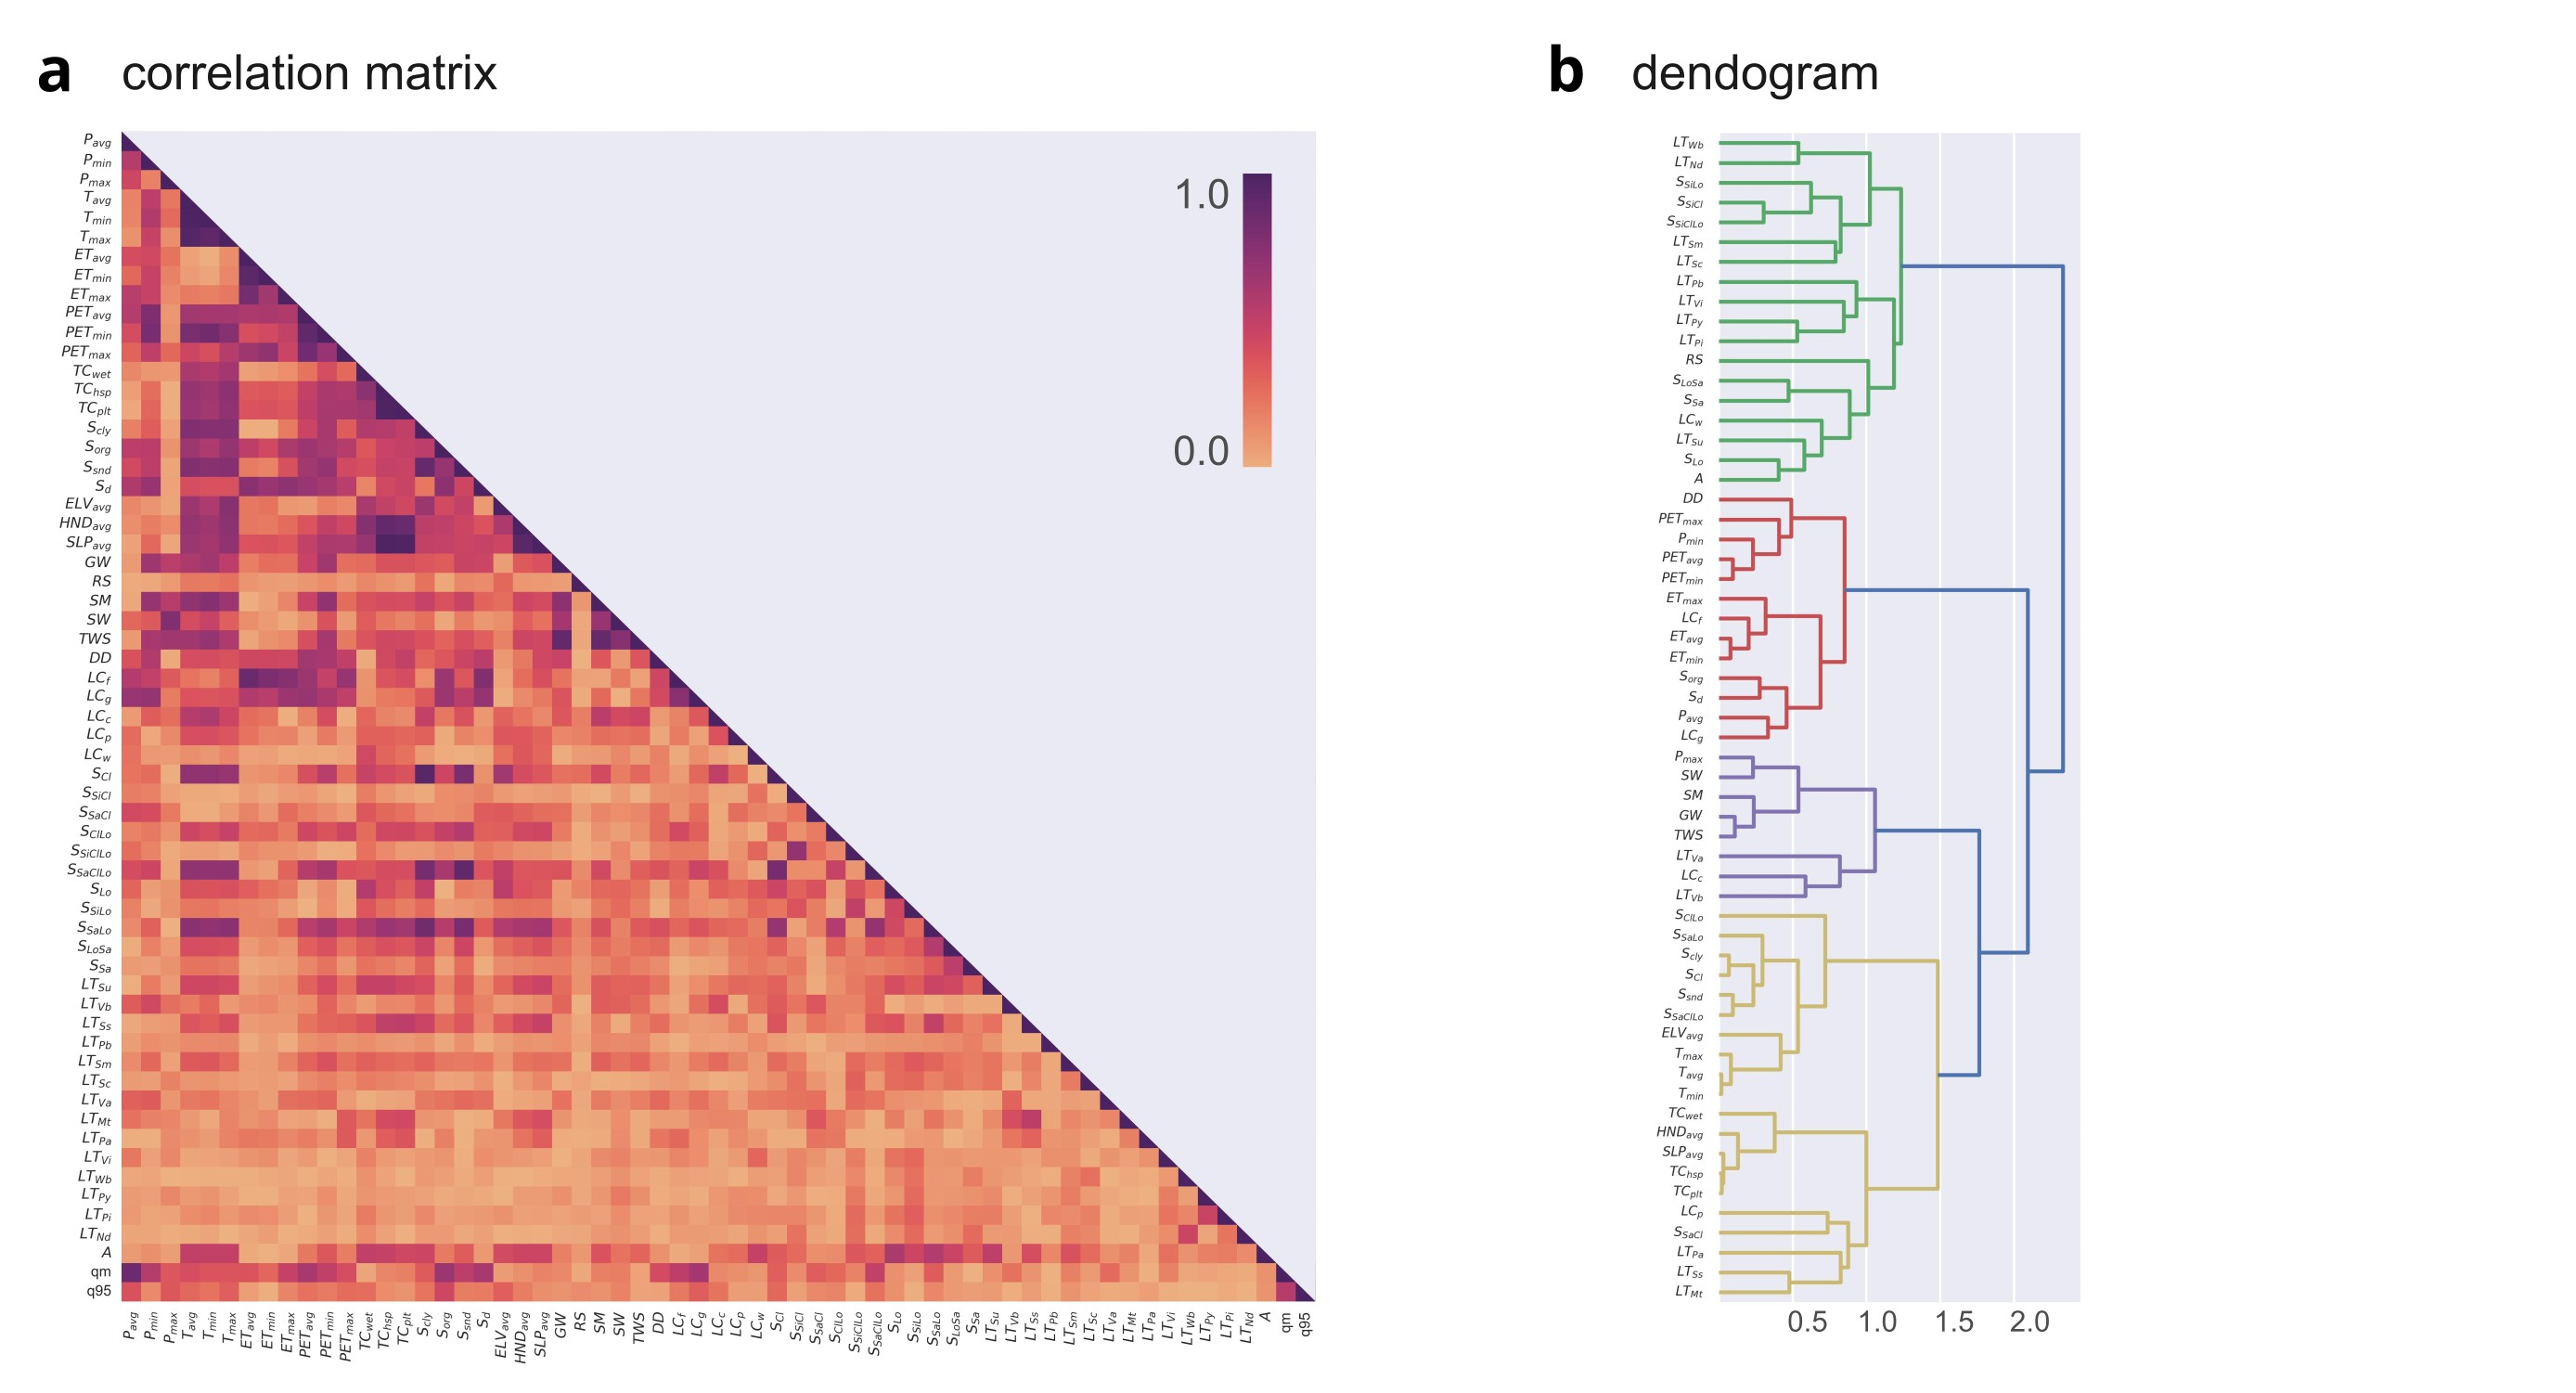
\includegraphics[width=0.98\linewidth]{figs/clusters.jpg}    
	\caption[Features correlation and clusters]
	{\textbf{---\;Feature analysis: correlation matrix and hierarchical clustering}.
	\textbf{a}\,--\,Correlation matrix, showing the absolute spearman correlation value, of the environmental predictors and target variables. 
        \textbf{b}\,--\,Dendogram representing the hierarchical relationship between the environmental predictors.
	}
    \label{fig:corrmatrix}            
\end{figure}

% Running times
\subsection{Running times}

\par Model complexity certainly plays a role in the time taken to run the algorithm. In Table \ref{tab:runtime}, the time to run all the setup presented in the model pipeline section for each model is presented, in a relatively simple desktop machine. Overall, comparing running times can give us a sense of the relative complexity of each model, but it's worth noting that the specific running time will depend on the size of the dataset, the complexity of the model, and the specific hyperparameters being used. \texttt{MLR} is the simplest model in the list and has the shortest running time by far, especially because this model doesn’t have hyperparameters to calibrate, which makes it even faster in the comparison. Other relatively time efficient model is \texttt{DT}, but still considerably more complex than linear regression. \texttt{KNN} and \texttt{SVM} come next in degree of complexity, taking between 2-4 minutes to run. Finally, \texttt{GBM} and \texttt{RF} are the most complex models in the list, which makes them considerably more computationally expensive than the other models, taking around 32 and 56 minutes, respectively.
% Insert Table 3
% Insert Table
\begin{table}[t]
\centering
\tiny
\rowcolors{2}{white}{rowgray}
\begin{tabular}{p{4cm}p{4cm}}
\toprule
\textbf{Model} & \textbf{Running time (mm:ss)}\\
\midrule
\texttt{MLR} & 00:02 \\
\texttt{DT}  & 00:14 \\
\texttt{KNN} & 02:28 \\
\texttt{SVM} & 04:01 \\
\texttt{GBM} & 31:57 \\
\texttt{RF}  & 55:53 \\
\bottomrule
\end{tabular}
\caption{Running times of each \texttt{ML} model.}
\label{tab:runtime}
\end{table}


% Performance evaluation
\subsection{Performance evaluation} \label{results:performance}

\begin{figure}[t!] % place figure in the page
	\centering                                       
	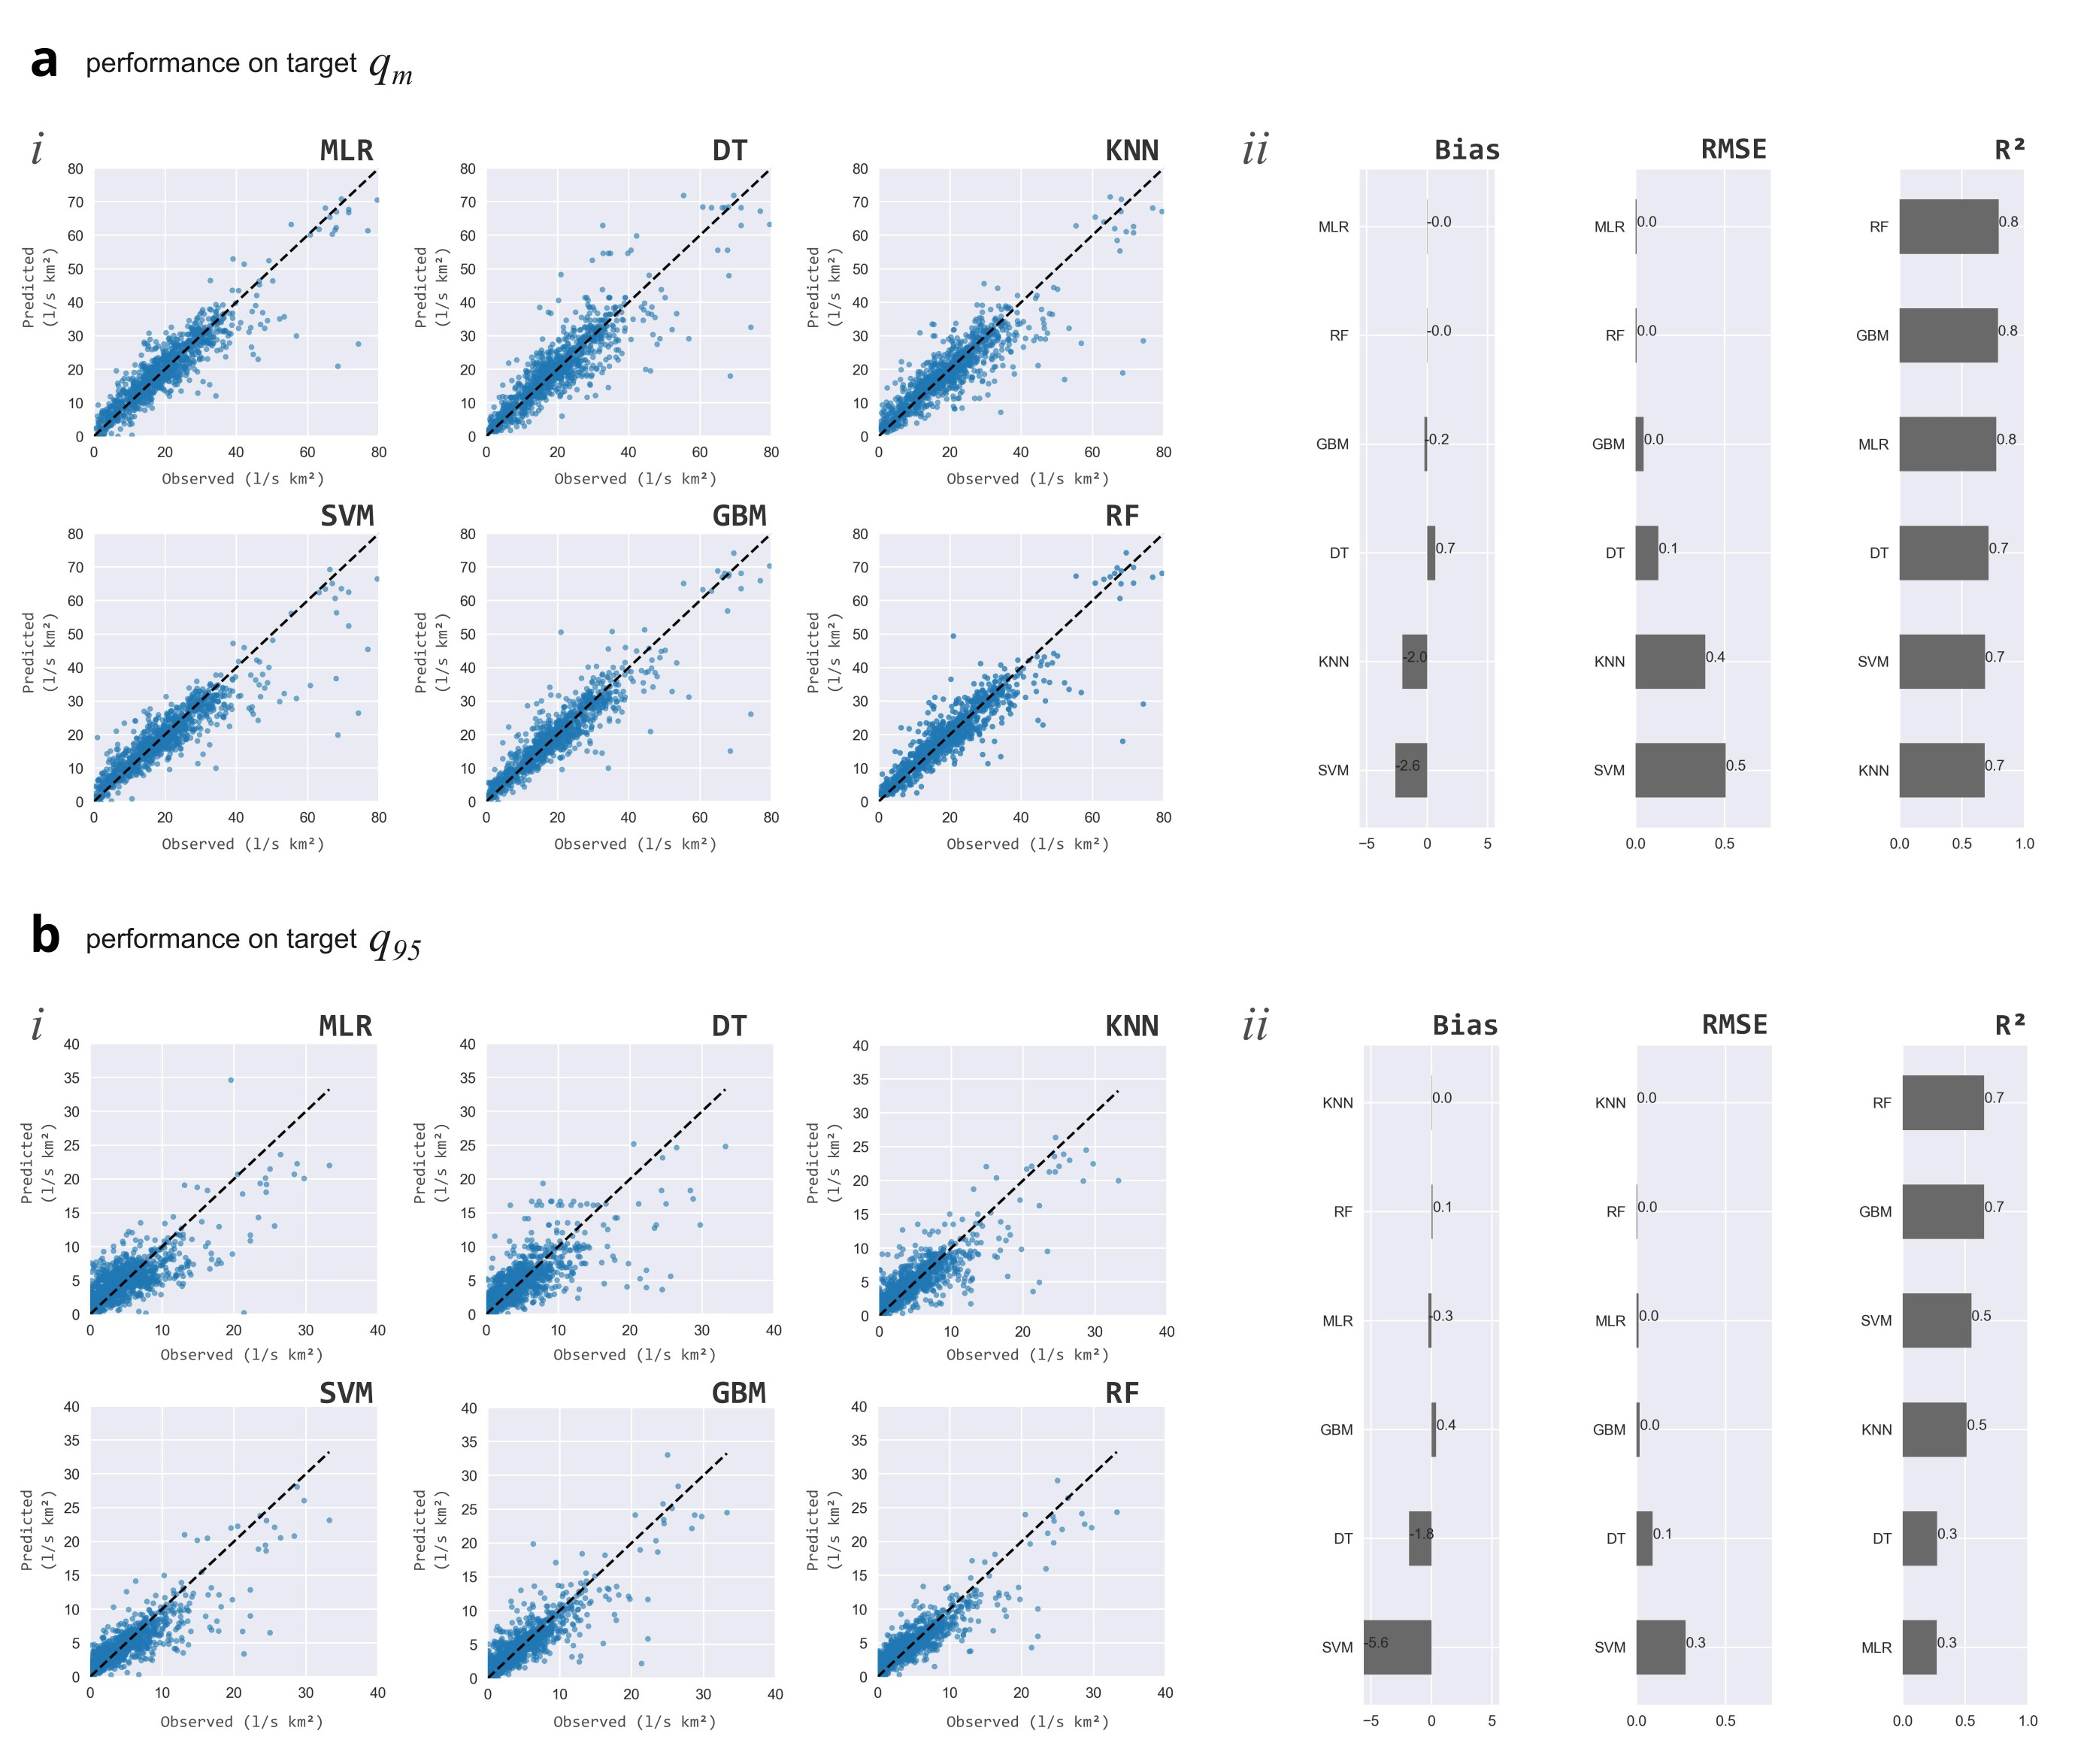
\includegraphics[width=0.98\linewidth]{figs/performance.jpg}    
	\caption[Performace of model evaluation]
	{ \textbf{---\;>>todo:legend Performace of \texttt{ML} model evaluation}.
		\textbf{a}\,--\,Tincidunt dui ut ornare lectus sit. Donec adipiscing tristique risus nec feugiat in fermentum posuere urna (detail \textrm{\textit{i}}).
		\textbf{b}\,--\,Tincidunt dui ut ornare lectus sit. Donec adipiscing tristique risus nec feugiat in fermentum posuere urna (detail \textrm{\textit{i}}).		
	}
	\label{fig:perf}  % use qualitative label                      
\end{figure}

\par The performance results of each \texttt{ML} model for $q_{m}$ and $q_{95}$ are presented in Figure 19 and Figure 20, respectively. \texttt{MLR} and \texttt{DT} had good overall performance in predicting $q_{m}$, with statistical metrics equivalent of those from the other models. These two models had similar bias and RMSE, with \texttt{MLR} having better performance in $R^2$ for $q_{m}$ (0.81 against 0.77), and \texttt{DT} for $q_{95}$ (0.55 against 0.48). However, despite having a reasonable performance for $q_{95}$, they were considerably worse in comparison with the other models, especially looking at $R^2$. Regarding the remaining models (\texttt{KNN}, \texttt{SVM}, \texttt{GBM} and \texttt{RF}), \texttt{KNN} presented the worse results overall for both variables, whereas \texttt{SVM}, \texttt{GBM} and \texttt{RF} presented similar results for both variables, with \texttt{SVM} having a more pronounced bias towards underestimation.

\par In summary, all models evaluated here presented reasonable performances for both variables. For $q_{95}$, the simpler benchmark models (\texttt{MLR} and \texttt{DT}) performed considerably worse, and \texttt{RF} had a slightly better performance than \texttt{GBM} and \texttt{SVM} overall. In $q_{m}$, the added complexity didn’t seem to improve much the performance, and even a simple model such as \texttt{MLR} had a performance equivalent to much more robust models, such as \texttt{GBM} and \texttt{RF}, for this variable.
% Insert Figure 5
% Insert Figure 6
% Importance of the predictors
\subsection{Importance of the predictors} \label{results:importance}

\begin{figure}[t!] % place figure in the page
	\centering                                       
	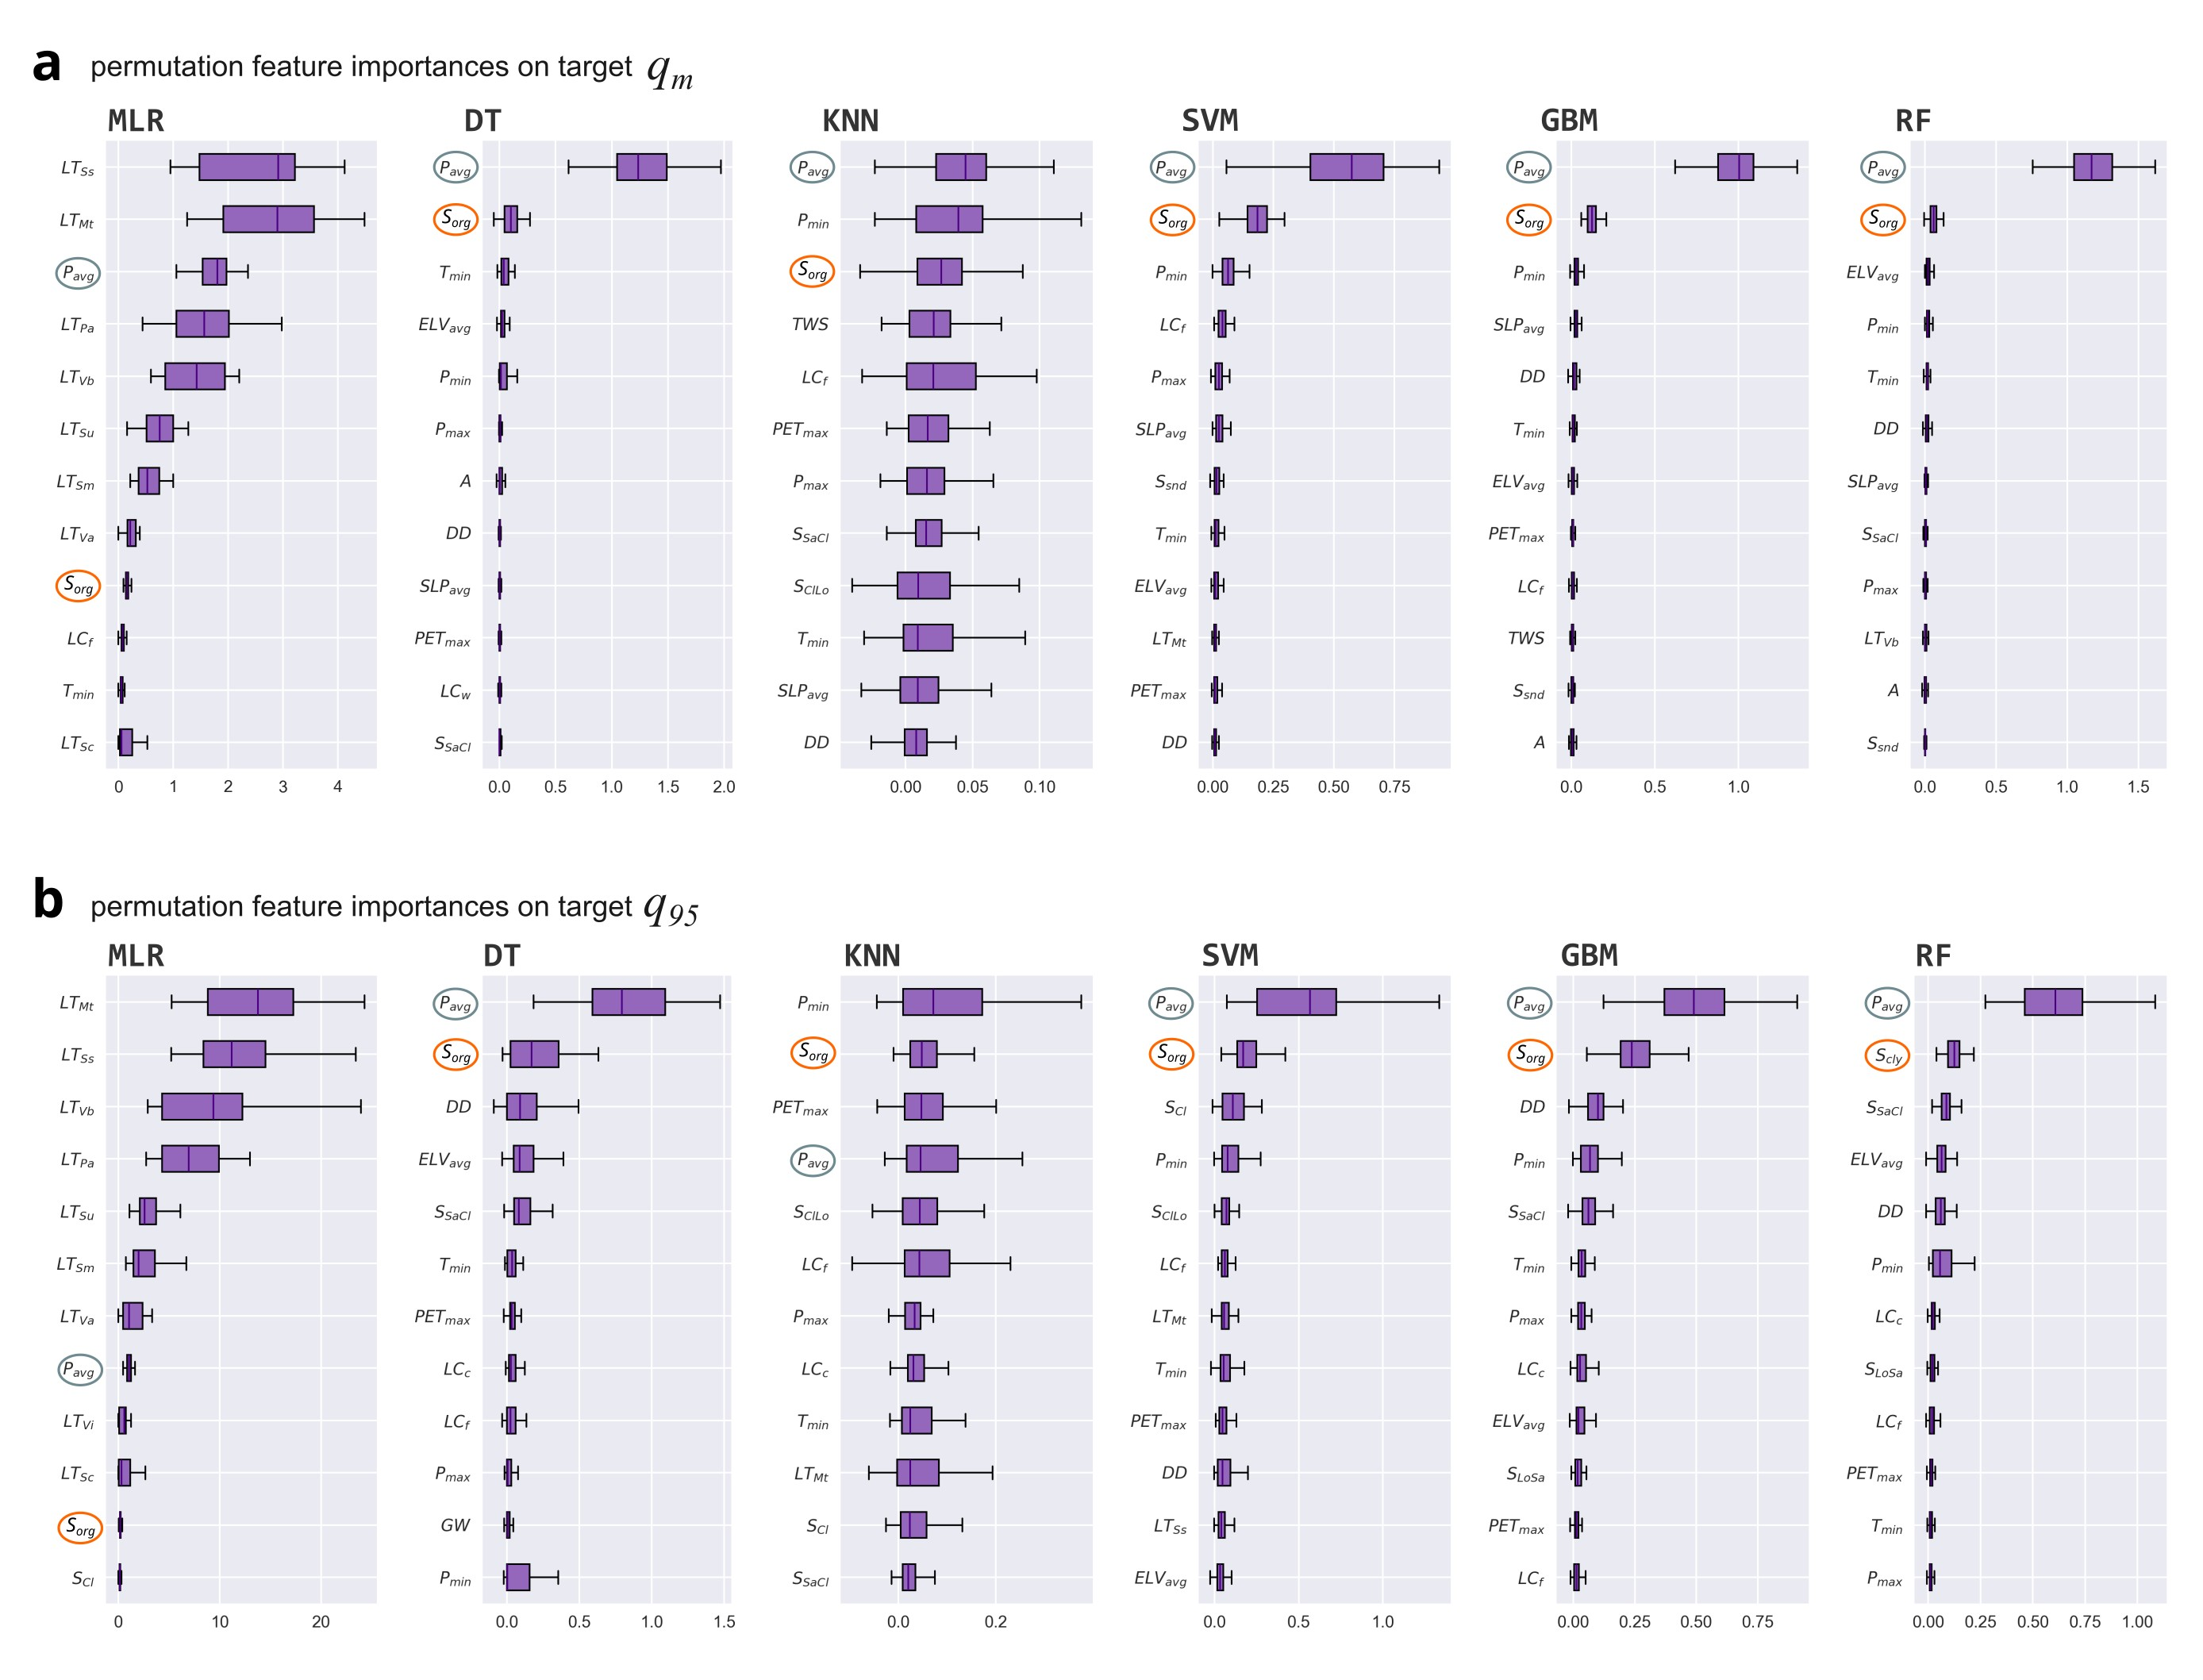
\includegraphics[width=0.98\linewidth]{figs/importance.jpg}    
	\caption[Importance of features]
	{ \textbf{---\;>>todo:legend}.
		\textbf{a}\,--\,Tincidunt dui ut ornare lectus sit. Donec adipiscing tristique risus nec feugiat in fermentum posuere urna (detail \textrm{\textit{i}}).
		\textbf{b}\,--\,Tincidunt dui ut ornare lectus sit. Donec adipiscing tristique risus nec feugiat in fermentum posuere urna (detail \textrm{\textit{i}}).		
	}
	\label{fig:importance}  % use qualitative label                      
\end{figure}

\par In Figure \ref{fig:importance} is presented the importances of the 12 most important features in each \texttt{ML} model for $q_{m}$ and $q_{95}$, respectively. The values reflect the decrease in $R^2$ value after randomly shuffling the selected variable. Overall, the average climatological precipitation ($p_{\text{avg}}$) was the most important predictor for all models and all target streamflow signatures. The importance of $p_{\text{avg}}$ is pronounced in most models, the only exception being the \texttt{KNN}, where variable weights in the results seem to be more evenly distributed for both target variables. Concerning all other models, for $q_{m}$, after $p_{\text{avg}}$ the other variables were much less important. Still, the organic content in soils ($soilorga$) had a meaningful contribution for the results, and other variables had mild contributions, such as average slope ($slp_{\text{avg}}$), average elevation ($elv_{\text{avg}}$), minimum climatological precipitation ($p_{\text{min}}$) and forest content ($lc_{\text{forest}}$). For $q_{95}$, despite $p_{\text{avg}}$ being still the most important predictor, its contribution is much less pronounced in comparison with other variables. Looking at \texttt{SVM}, \texttt{GBM} and \texttt{RF}, which were the best performing models for $q_{95}$, we can see large contributions of $soilorga$, $p_{\text{min}}$ and $elv_{\text{avg}}$ in addition to the content of sand-clay ($st_{\text{SaCl}}$, for \texttt{GBM} and \texttt{RF}) and clay ($st_{\text{Cl}}$, for \texttt{SVM}) textures. It’s worth mentioning that these variables are the representative variables from the hierarchical cluster selection (Figure 18), so the premise is that the models would have similar performances and importances if using any of the variables in the respective cluster.

% Uncertainty analysis
\subsection{Uncertainty insights} \label{results:uncert}

\begin{figure}[t!] % place figure in the page
	\centering                                       
	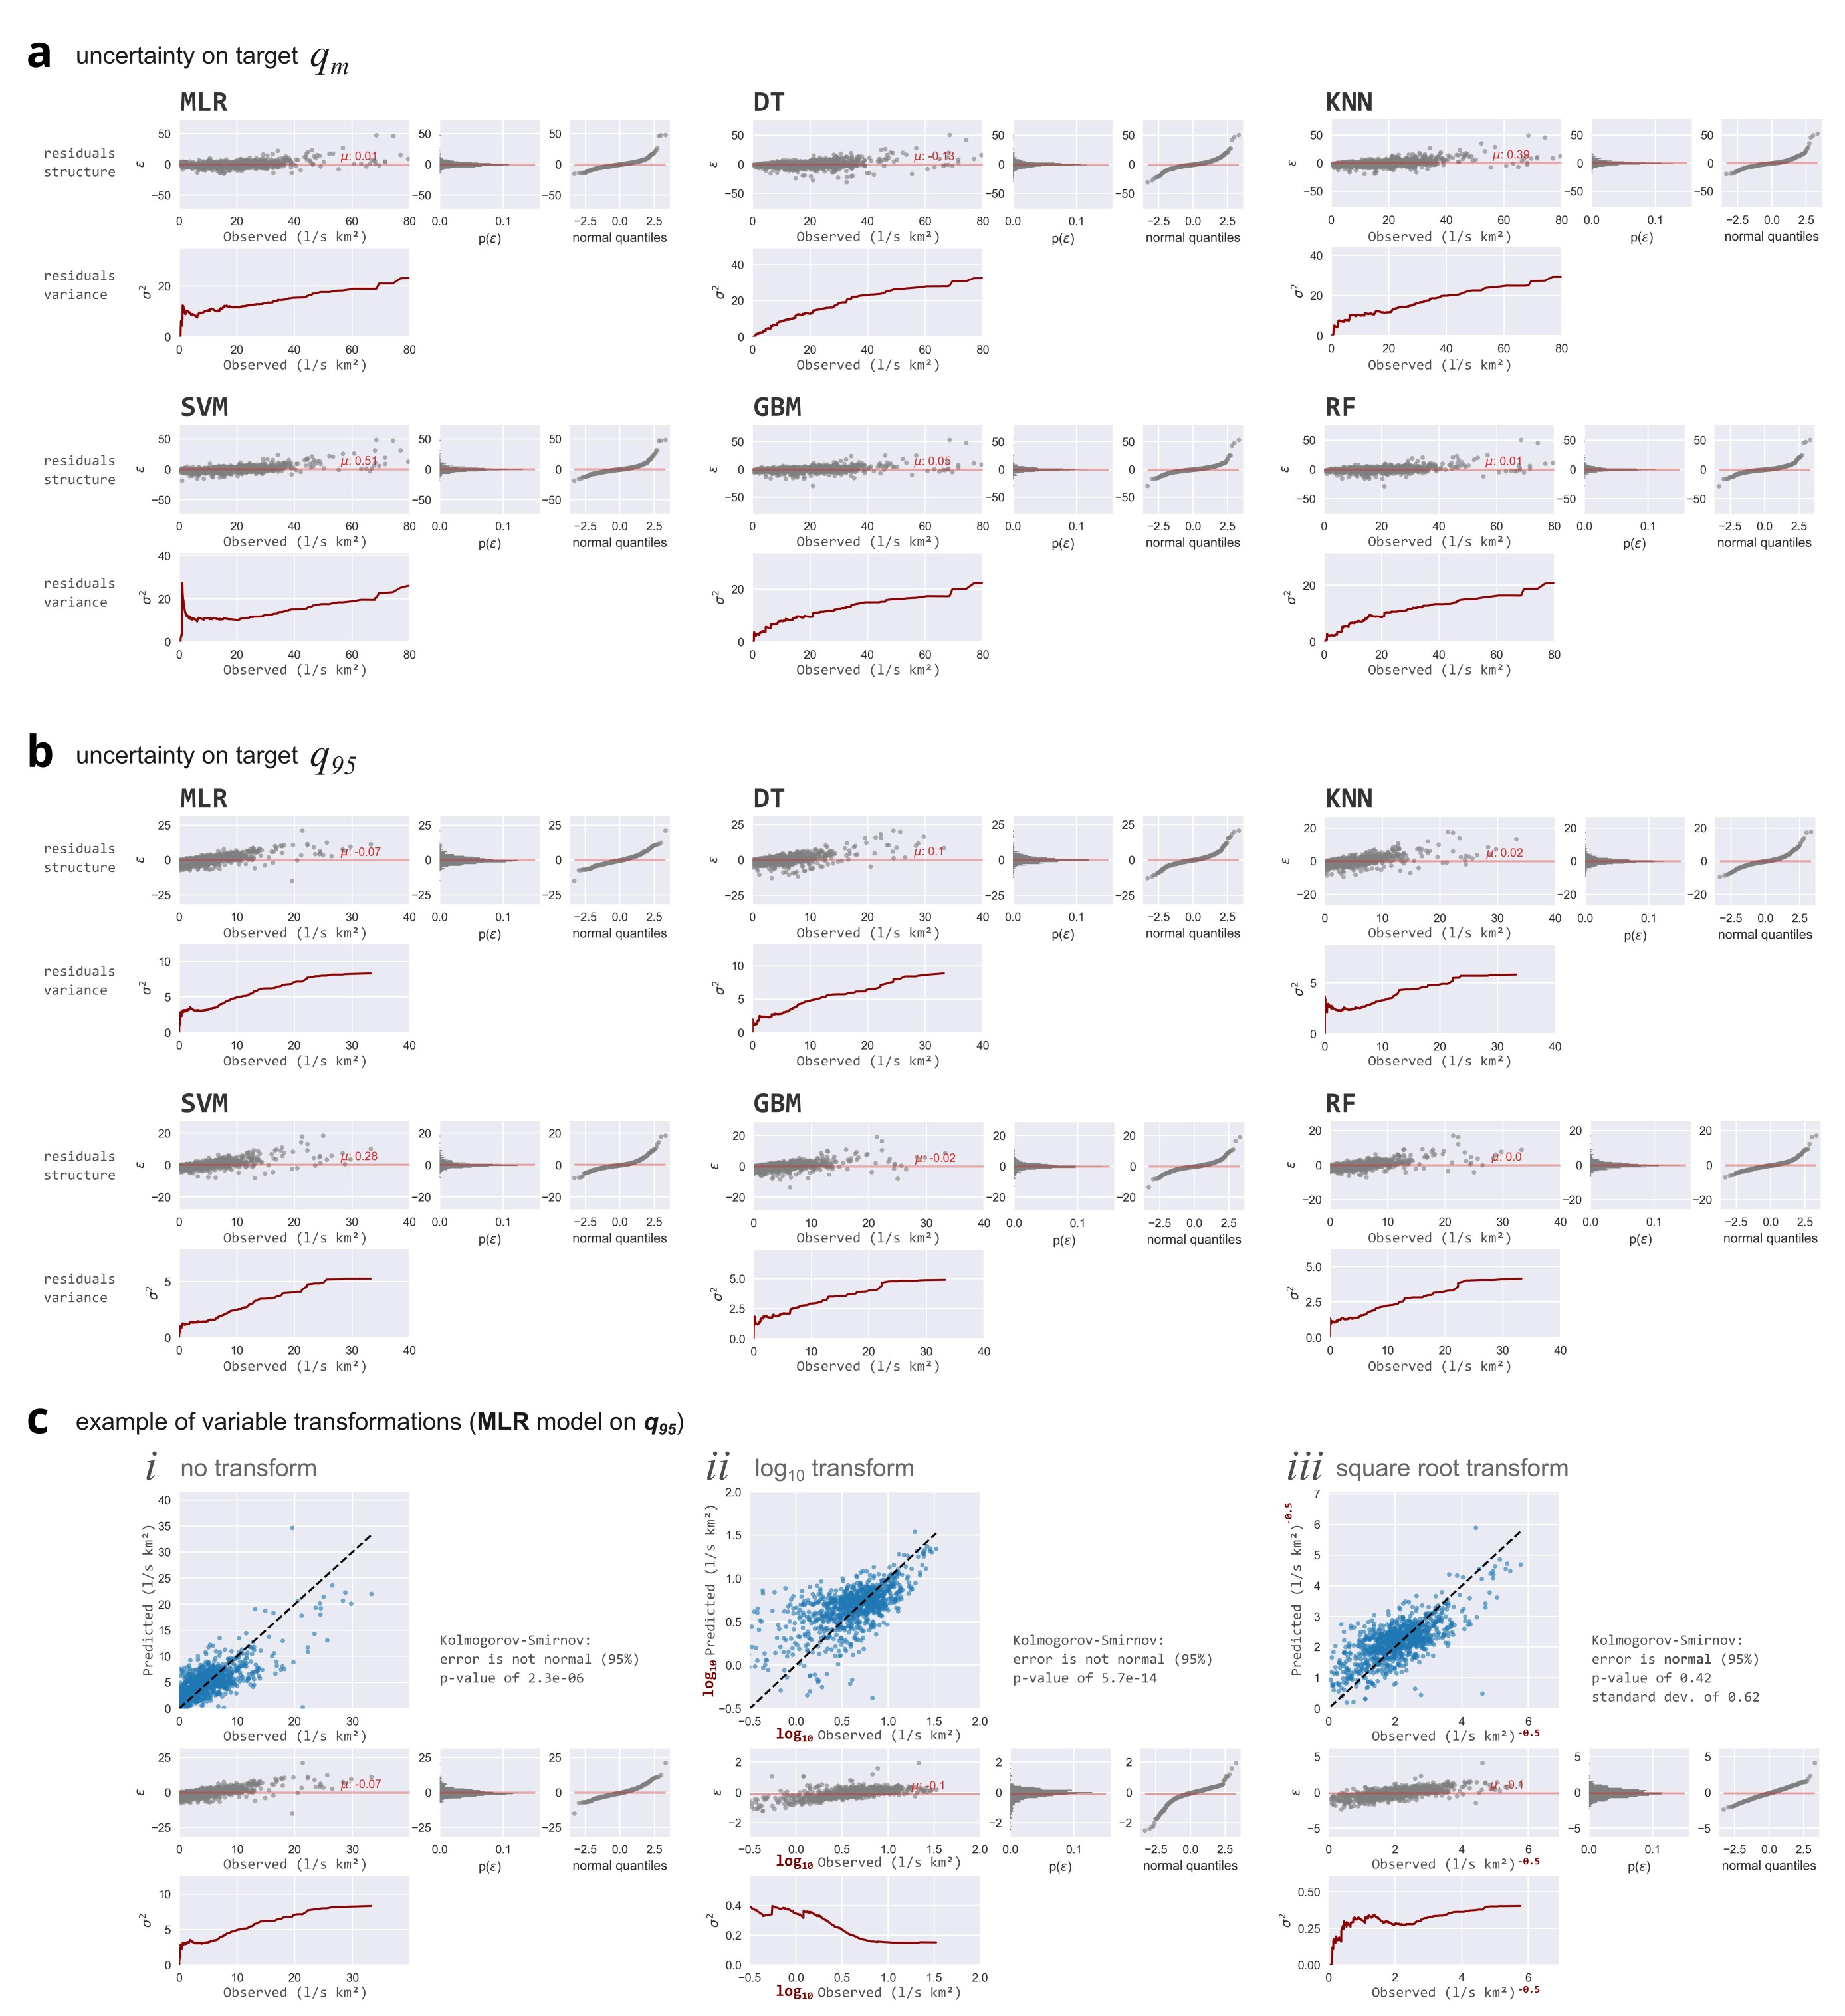
\includegraphics[width=0.98\linewidth]{figs/uncertainty.jpg}    
	\caption[Insights into Uncertainty]
	{\textbf{---\;Insights into Uncertainty from Residuals Analysis}.
        \textbf{a}\,--\,Analysis of uncertainty for the target variable $q_m$, revealing the structure of residuals $\epsilon$ (including distribution, histogram, and Quantile-Quantile plot) and examining the stability of accumulated variance $\sigma^2$ for each Machine Learning model.
        \textbf{b}\,--\,Analysis of uncertainty for the target variable $q_{95}$, revealing the structure of residuals $\epsilon$ (including distribution, histogram, and Quantile-Quantile plot) and examining the stability of accumulated variance $\sigma^2$ for each Machine Learning model.
        \textbf{c}\,--\,Variable transformations applied in the \texttt{MLR} model for the target variable $q_{95}$ included: no transformation (detail \textrm{\textit{i}}); logarithmic transformation (detail \textrm{\textit{ii}}); and square root transformation (detail \textrm{\textit{iii}}). The square root transformation was the only method that passed the Kolmogorov-Smirnov test.
        }
	\label{fig:uncert}  % use qualitative label                      
\end{figure}

\par The assessment of uncertainty in fitting models to target variables $q_{m}$ and $q_{95}$ provided various insights into the distribution and structure of errors. The panels in Figure \ref{fig:uncert}a and Figure \ref{fig:uncert}b display the visualizations used for all six machine learning models adjusted for target variables $q_{m}$ and $q_{95}$, respectively. In each model, the first three charts visually present the structure of the residuals: the first chart shows the residuals as a function of the magnitude of the observed variable, the second is a histogram of the residuals, and the third is the Quantile-Quantile plot, which relates the empirical quantiles obtained with the expected quantiles for a normal distribution. The fourth chart, vertically aligned with the residual chart, depicts the accumulated variance $\sigma^2$ as a function of the magnitude of observed values. This visualization is particularly informative, as if the residuals emerge from a random process (i.e., with independence), the variance should quickly stabilize around a constant value as the number of samples increases.

\par The residual structure charts reveal that the residuals are relatively well-centered around zero, with generally very low means (the highest value for the mean was 0.51 l/s km$^2$ for the \texttt{SVM} model on the $q_m$ target variable). However, this symmetry in the mean does not imply structural symmetry, as positive residuals tend to be larger for higher observed values, indicating that the machine learning models generally underestimate higher reference flows. The Quantile-Quantile charts reinforce this observation, as the upper tail mostly presents a more pronounced curve, reaching higher values (around 50 l/s km$^2$) on the positive side. Notably, the residuals of the \texttt{MLR} model on the $q_{95}$ target variable showed the most random-like structure, with a highly symmetric distribution, as demonstrated by the nearly straight-line Quantile-Quantile plot.

\par The cumulative variance charts highlight the fact that none of the model residuals showed stability, with all charts being a gradually increasing curve. The observed heteroscedasticity in the fits suggests that the errors in the models have a multiplicative nature, rather than additive. Even though the modeled flows here are normalized by drainage area, this finding aligns with available theory on fitting rating-curves (\cite{Mcmillan2015}), with the uncertainty of higher values being disproportionately larger. Reasons for this include statistical uncertainties, such as the low sample number of high flows due to technical difficulties and the uncertainty of available measurement methods, as well as epistemic uncertainties, such as floodplain geometry, hydraulic model , etc. In this context, our results suggest that the machine learning models may be contaminated with this form of observational uncertainty. Another explanation, not mutually exclusive with the former, could be that incrementally higher specific flows indicate an incrementally lower control capacity of the environmental factors considered in attenuating climatic variabilities, such as in watersheds with very shallow soils.

\par Variable transformations (logarithm and square root) thus allowed for the assessment of alternative structures to stabilize the variance of the residuals. The results of the transformations substantially improved the error distribution, evident by more straight-line-like Quantile-Quantile charts. Nonetheless, Kolmogorov-Smirnov tests applied (including without transformation) indicated that only the \texttt{MLR} model on the target variable $q_{95}$ showed a normal distribution with 95\% confidence in the case of the square root transformation, as illustrated in Figure \ref{fig:uncert}c (detail \textit{ii}). In this case, the standard deviation of the normal distribution was obtained at 0.62 (l/s km$^2$)$^{-0.5}$, a value that can be used in Monte Carlo simulations and re-transformed back to the target variables of the machine learning models.

\par >>todo: evaluate presenting old results

\par \textcolor{red}{The preliminary results for uncertainty are shown in Figure 23 and Figure 24, only for \texttt{GBM} and \texttt{RF}, which are the models that presented the best performance, although it didn’t differ much for the rest of the models analyzed. The \texttt{CV+} method was able to capture a coverage of $>95\%$, as the theoretical description suggested, although the values are still very high and constant for all value magnitudes, with $q_{m}$ uncertainty around 20 l/s and $q_{95}$ around 10 l/s. This high uncertainty doesn’t reflect the performance of the models in predicting the variables, and other methodologies will be tested to fill this gap, perhaps with the caveat of reducing the coverage.}

% Dataset covering all Brazilian unit catchments
\subsection{Dataset covering all Brazilian unit catchments} \label{results:dataset}

\par A dataset was produced by extrapolating the results of the models produced to cover all Brazilian catchments.

\par \textcolor{red}{Nam blandit dui quis nunc pretium, sed egestas felis mattis. Aenean tristique, massa non vestibulum pulvinar, justo ante efficitur turpis, vitae feugiat sem nisi ut arcu. Lorem ipsum dolor sit amet, consectetur adipiscing elit. Nunc rhoncus lacus nisi, id efficitur ligula placerat quis. Maecenas sit amet mi aliquam, congue metus a, accumsan leo. Vivamus id lobortis libero, ac fermentum ligula. In sollicitudin, enim varius rhoncus feugiat, odio lectus interdum enim, a posuere nunc magna eget nisi. Sed eget lacus et ante mollis sollicitudin quis varius velit. Aenean sit amet ipsum rhoncus eros iaculis ornare. Phasellus nec tortor ultrices orci sollicitudin fermentum. Mauris mattis nibh dui, a condimentum mi fermentum sed. Aliquam ac tempor mi. Fusce ac libero pharetra, sagittis metus id, dictum massa. Vestibulum ante ipsum primis in faucibus orci luctus et ultrices posuere cubilia curae; Sed a erat accumsan, interdum leo sed, porttitor risus.}

% Discussion and conclusions
\section{Discussion and conclusions} \label{discussion}
% Limitations
\subsection{Limitations} \label{discussion:limitations}

\par \textcolor{red}{Hypsometry of catchments
Uncertainty in data (target discharges and environmental)}


\par \textcolor{red}{Nam blandit dui quis nunc pretium, sed egestas felis mattis. Aenean tristique, massa non vestibulum pulvinar, justo ante efficitur turpis, vitae feugiat sem nisi ut arcu. Lorem ipsum dolor sit amet, consectetur adipiscing elit. Nunc rhoncus lacus nisi, id efficitur ligula placerat quis. Maecenas sit amet mi aliquam, congue metus a, accumsan leo. Vivamus id lobortis libero, ac fermentum ligula. In sollicitudin, enim varius rhoncus feugiat, odio lectus interdum enim, a posuere nunc magna eget nisi. Sed eget lacus et ante mollis sollicitudin quis varius velit. Aenean sit amet ipsum rhoncus eros iaculis ornare. Phasellus nec tortor ultrices orci sollicitudin fermentum. Mauris mattis nibh dui, a condimentum mi fermentum sed. Aliquam ac tempor mi. Fusce ac libero pharetra, sagittis metus id, dictum massa. Vestibulum ante ipsum primis in faucibus orci luctus et ultrices posuere cubilia curae; Sed a erat accumsan, interdum leo sed, porttitor risus.}

% Performance of the models and environmental data
\subsection{Performance of the models and environmental data} \label{discussion:performance}

\par The results suggest that machine learning models can be effective in predicting streamflow for both $q_{m}$ and $q_{95}$, and also highlight the importance of carefully selecting and tuning the models to achieve optimal performance, as well as the need for high-quality data to feed them. The performance of the models can vary depending on the specific model used. More robust models, such as \texttt{GBM} and \texttt{RF}, had similar results than simpler models such as \texttt{MLR} or \texttt{DT} for $q_{m}$, and only slightly better results for $q_{95}$ when comparing with a much less complex \texttt{SVM}. For $q_{95}$, in particular, the simplicity of \texttt{MLR}, \texttt{DT} and \texttt{KNN} yield reasonable results, with $R^2$ between 0.48 to 0.66, although a quite significant improvement was achieved with \texttt{SVM} (with $R^2$ of 0.74), and an improvement in bias by the incremented complexity of \texttt{GBM} and \texttt{RF}.

\par Regarding the importance of the variables, it’s not surprising that average precipitation is the most important predictor overall. Still, for the case of predicting low flows ($q_{95}$), other variables deserve to be highlighted, as they presented meaningful contributions in predicting the results, they are (grouped by cluster):
\begin{itemize}
\item Organic content in soils and/or soil density
\item Average elevation and/or wetland occupation rate
\item Minimum precipitation, average/minimum/maximum $PET$ and/or drainage density
\item Sand-clay texture occupation rate
\end{itemize}

\par The fact that these variables were grouped this way is not always obvious, nor why they were so important in the $q_{95}$ prediction. The main assumption with the process of hierarchical clustering is that one variable of the cluster can be used to predict the other(s), and that the selection of any of the variables from the cluster wouldn’t yield significantly different results, because all variables within a cluster are highly correlated. Of course, the distance criterion for cluster separation is subject to analysis, and our criterion here was that no selected variable would have pair-wise spearman correlation above 0.7. Still, it wasn’t tested whether (1) using different thresholds would result in different model performances, nor (2) using a different variable from each cluster would impact the results.

% Comparison with previous studies
\subsection{Comparison with previous studies} \label{discussion:previous}

\par As the use of machine learning models is quite recent in hydrology research, only three studies that attempted to use \texttt{ML} models to predict streamflow signatures were found: one for peak event flows over the United States (\cite{potdar2021}), one for low flows comprising around 200 basins in the southern USA (\cite{worland2018}), and one for average and low flows in the Doce River basin in Brazil ( \cite{ferreira2021}). There are a few points that are worth discussing about these studies in relation to the one presented herein, regarding mostly the model inter-comparisons and the process of feature selection and importance computation.

\par In the two studies that compared the performances of linear models, such as \texttt{MLR}, with more robust state-of-the-art \texttt{ML} models (\cite{ferreira2021, worland2018}), both found the predictions of linear models being much worse than more complex models, which is contrasting with the results found here, where a linear structure was similar to a more complex structures for mean flows, and only worse for low flows albeit having reasonable estimates. Both studies used similar environmental predictors, as well as of cross-validation and hyperparameter tuning, with small differences in comparison with this study. The main difference relies on the process of filtering the data that is being used by the models. Still, the process of feature selection shouldn’t be the reason for considerable decrease in performance, as this process is performed with the main goals of reducing running times and removing multi-collinearity for later assessing variable importances.

\par Regarding the importances of the predictors, in all three studies mentioned in this discussion this process is performed without the adequate feature selection to reduce multi-collinearity. Reducing multi-collinearity is essential for feature importance computation, because if there are two correlated variables, one will compensate for the absence of the other, and so both of them will have their importances drastically underestimated. Despite that, in \cite{worland2018} and \cite{potdar2021}, no process of feature selection is performed. In \cite{ferreira2021}, the authors removed variables with pair-wise pearson correlation below 0.95, which is a very high threshold (recommended values in the literature vary from 0.6 to 0.8), and later performed recursive feature elimination (RFE), which is a process that requires importance computation to remove non-important features, and should only be performed in non-collinear data. Because of those methodological flaws, all analyses regarding variable importances in those studies won’t be considered for comparison with this study.

% General recommendations
\subsection{General recommendations} \label{discussion:recommend}

Based on the investigation carried in this study, a few recommendations for the use of machine learning for predicting streamflow in ungauged catchments are given:
\begin{itemize}
    \item For predicting average streamflow, the complexity of the model used doesn’t yield a significant improvement in the results, and average precipitation alone could give reasonable estimates.
\end{itemize}

\begin{itemize}
    \item For low flows, besides average precipitation, other data become more important, such as soil organic content, minimum precipitation and elevation; and more robust non-linear models have a better performance.
\end{itemize}

\begin{itemize}
    \item The quality of environmental data is the most valuable asset for such applications, regardless of the model. As these applications were made very easy by recent developments, studies should focus more on targeting the preparation and investigation of the data. Processes such as multi-collinearity analysis and feature selection should receive more attention, which is not the case in most studies to date.
\end{itemize}

\section*{CRediT authorship contribution statement}

\noindent 
>>todo: credits
\textbf{Rafael Barbedo}: Project administration, Funding acquisition, Conceptualization, Supervision, Methodology, Writing – original draft. \textbf{Iporã Possantti}: Investigation, Visualization, Formal analysis, Writing – review and editing. \textbf{Author C}: Investigation, Formal analysis. \textbf{Author C}: Investigation, Formal analysis. \textbf{Author C}: Investigation, Formal analysis.

\section*{Data availability}

\noindent Data will be made available on request. >>todo: links and more options.

\section*{Acknowledgements}

\noindent \par The authors would like to acknowledge the financial support provided by the Brazilian National Water and Sanitation Agency (ANA) in the context of the project \say{Technological Cooperation for Hydrological Assessments in Brazil — Streamflow regionalisation} (grant number: TED-05/2019-ANA), the Google LLC for making available the Google Earth Engine (GEE) platform, and all data providers for the global products used in this study.

\section*{Declaration on competing interest}

\noindent The authors declare that they have no known competing financial interests or personal relationships that could have appeared to influence the work reported in this paper.

\section*{Declaration of generative AI and AI-assisted technologies}

\noindent During the preparation of this work the authors used \texttt{CHAT-GPT 4.0} in order to improve language and readability. After using this tool, the authors reviewed and edited the content as needed and take full responsibility for the content of the publication.

	
% ---------------- Appendix ----------------
\clearpage
\begin{appendices}
	
\section{The Appendix} \label{ap:first}

\par >>todo: appendix -- database figure(s) and description.

\par \textcolor{red}{Nam blandit dui quis nunc pretium, sed egestas felis mattis. Aenean tristique, massa non vestibulum pulvinar, justo ante efficitur turpis, vitae feugiat sem nisi ut arcu. Lorem ipsum dolor sit amet, consectetur adipiscing elit. Nunc rhoncus lacus nisi, id efficitur ligula placerat quis. Maecenas sit amet mi aliquam, congue metus a, accumsan leo. Vivamus id lobortis libero, ac fermentum ligula. In sollicitudin, enim varius rhoncus feugiat, odio lectus interdum enim, a posuere nunc magna eget nisi. Sed eget lacus et ante mollis sollicitudin quis varius velit. Aenean sit amet ipsum rhoncus eros iaculis ornare. Phasellus nec tortor ultrices orci sollicitudin fermentum. Mauris mattis nibh dui, a condimentum mi fermentum sed. Aliquam ac tempor mi. Fusce ac libero pharetra, sagittis metus id, dictum massa. Vestibulum ante ipsum primis in faucibus orci luctus et ultrices posuere cubilia curae; Sed a erat accumsan, interdum leo sed, porttitor risus.}

\begin{figure}[t!] % place figure in the page
	\centering                                       
	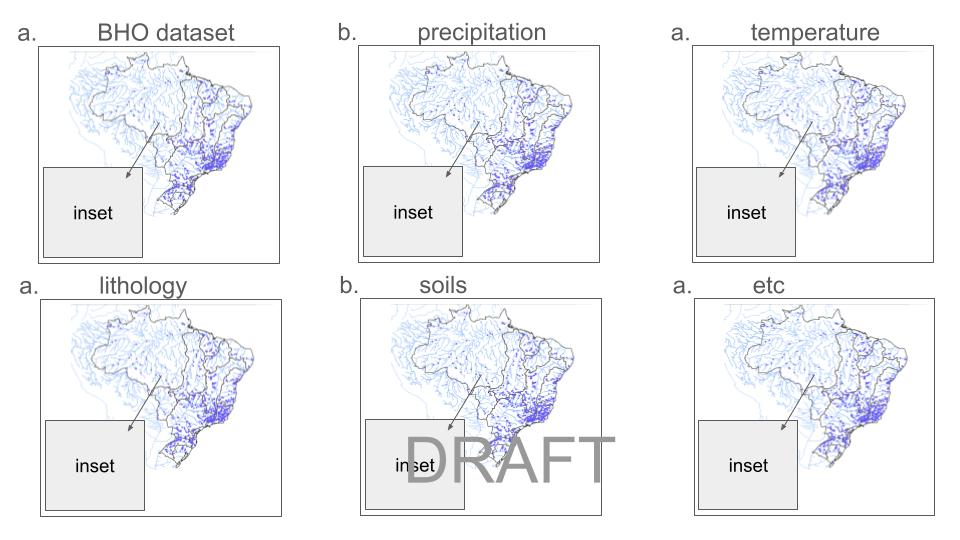
\includegraphics[width=0.98\linewidth]{figs/pre_descrip.jpg}    
	\caption[>>:todo:caption Short caption]
	{ \textbf{---\;>>todo:caption This is the long caption}.
		\textbf{a}\,--\,Tincidunt dui ut ornare lectus sit. Donec adipiscing tristique risus nec feugiat in fermentum posuere urna (detail \textrm{\textit{i}}).
		\textbf{b}\,--\,Tincidunt dui ut ornare lectus sit. Donec adipiscing tristique risus nec feugiat in fermentum posuere urna (detail \textrm{\textit{i}}).		
	}
	\label{fig:descript}  % use qualitative label                      
\end{figure}


\clearpage

\end{appendices}
% print references
\clearpage
\singlespacing
\printbibliography
\end{document}
	
